%%%%%%%%%%%%%%%%%%%%%%%%%%%%%%%%%%%%%%%%%
% Masters/Doctoral Thesis 
% LaTeX Template
% Version 2.5 (27/8/17)
%
% This template was downloaded from:
% http://www.LaTeXTemplates.com
%
% Version 2.x major modifications by:
% Vel (vel@latextemplates.com)
%
% This template is based on a template by:
% Steve Gunn (http://users.ecs.soton.ac.uk/srg/softwaretools/document/templates/)
% Sunil Patel (http://www.sunilpatel.co.uk/thesis-template/)
%
% Template license:
% CC BY-NC-SA 3.0 (http://creativecommons.org/licenses/by-nc-sa/3.0/)
%
%%%%%%%%%%%%%%%%%%%%%%%%%%%%%%%%%%%%%%%%%

%----------------------------------------------------------------------------------------
%	PACKAGES AND OTHER DOCUMENT CONFIGURATIONS
%----------------------------------------------------------------------------------------



\documentclass[
11pt, % The default document font size, options: 10pt, 11pt, 12pt
%oneside, % Two side (alternating margins) for binding by default, uncomment to switch to one side
english, % ngerman for German
singlespacing, % Single line spacing, alternatives: onehalfspacing or doublespacing
%draft, % Uncomment to enable draft mode (no pictures, no links, overfull hboxes indicated)
%nolistspacing, % If the document is onehalfspacing or doublespacing, uncomment this to set spacing in lists to single
%liststotoc, % Uncomment to add the list of figures/tables/etc to the table of contents
%toctotoc, % Uncomment to add the main table of contents to the table of contents
%parskip, % Uncomment to add space between paragraphs
%nohyperref, % Uncomment to not load the hyperref package
headsepline, % Uncomment to get a line under the header
%chapterinoneline, % Uncomment to place the chapter title next to the number on one line
%consistentlayout, % Uncomment to change the layout of the declaration, abstract and acknowledgements pages to match the default layout
]{MastersDoctoralThesis} % The class file specifying the document structure

\usepackage[utf8]{inputenc} % Required for inputting international characters
\usepackage[T1]{fontenc} % Output font encoding for international characters

\usepackage{mathpazo} % Use the Palatino font by default


\usepackage[
backend =bibtex,
natbib=true,
style=numeric,
sorting=none]{biblatex}


%\usepackage[sorting = none, backend=bibtex]{biblatex} % Use the bibtex backend with the authoryear citation style (which resembles APA)

%\bibliographystyle{ieeetr})

\addbibresource{example.bib} % The filename of the bibliography



\usepackage[autostyle=true]{csquotes} % Required to generate language-dependent quotes in the bibliography

\usepackage{xcolor} %Change text color

\usepackage{siunitx} %math symbol

\usepackage{hyperref} %references

\usepackage{bm} %bold font

\setcounter{secnumdepth}{4} %subsubsection and so on

%Path to inkscape folder
\makeatletter
\def\input@path{{/Users/gabrielsuc/Documents/Bang_Olufsen/Report/InkScape/}}
%or: \def\input@path{{/path/to/folder/}{/path/to/other/folder/}}
\makeatother

\usepackage{amsmath} %equation
\usepackage{amssymb}

%subfigures
\usepackage[format=hang]{caption}
\usepackage{subcaption}
\captionsetup[subfigure]{labelfont=rm}
\usepackage{float}

%matlab
\usepackage{xspace}
\newcommand{\MATLAB}{\textsc{Matlab}\xspace}

 %split equation over pages
\allowdisplaybreaks

%Justify text inside paragraph
\usepackage{ragged2e}

%Change size of math symbols
\usepackage{relsize}

%Item with numbers
\usepackage{enumitem}
%\newlist{legal}{enumerate}{10}
%\setlist[legal]{label*=\arabic*.}


\setlist[enumerate]{wide=0pt, widest=99,leftmargin=\parindent, labelsep=* } 
%tikz
\usepackage{tikz}
\usepackage{tikz-dsp}
\tikzset{rounded corners=0}
\usetikzlibrary{decorations.pathreplacing}

\usepackage{slashbox}

%footnote
\usepackage[bottom]{footmisc}

%handle figure + table
\usepackage{placeins}

\usepackage{graphics}

\usepackage{multirow}

\usepackage{array}

\newcommand\ChangeRT[1]{\noalign{\hrule height #1}}

%----------------------------------------------------------------------------------------
%	MARGIN SETTINGS
%----------------------------------------------------------------------------------------

\geometry{
	paper=a4paper, % Change to letterpaper for US letter
	inner=2.5cm, % Inner margin
	outer=3.8cm, % Outer margin
	bindingoffset=.5cm, % Binding offset
	top=1.5cm, % Top margin
	bottom=1.5cm, % Bottom margin
	%showframe, % Uncomment to show how the type block is set on the page
}

%----------------------------------------------------------------------------------------
%	THESIS INFORMATION
%----------------------------------------------------------------------------------------

\thesistitle{Real-Time Sample Rate Converter for High-Quality Audio Signal Processing} % Your thesis title, this is used in the title and abstract, print it elsewhere with \ttitle
\supervisor{Dr. Pablo \textsc{Martínez-Nuevo}\\
Dr. Sven Ewan \textsc{Shepstone}\\
Mr. Henrik Lund \textsc{Jensen}\\
Dr. Geoff \textsc{Martin}} % Your supervisor's name, this is used in the title page, print it elsewhere with \supname
\examiner{Dr. Matthieu \textsc{Guerquin-Kern}} % Your examiner's name, this is not currently used anywhere in the template, print it elsewhere with \examname
\degree{Electrical Engineer} % Your degree name, this is used in the title page and abstract, print it elsewhere with \degreename
\author{Gabriel \textsc{Suc}} % Your name, this is used in the title page and abstract, print it elsewhere with \authorname
\addresses{} % Your address, this is not currently used anywhere in the template, print it elsewhere with \addressname

\subject{} % Your subject area, this is not currently used anywhere in the template, print it elsewhere with \subjectname
\keywords{} % Keywords for your thesis, this is not currently used anywhere in the template, print it elsewhere with \keywordnames
\university{\href{http://www.ensea.fr/en}{Ecole Nationale Supérieure de l'Electronique et de ses Applications}} % Your university's name and URL, this is used in the title page and abstract, print it elsewhere with \univname
\department{\href{}{Multimedia Systems}} % Your department's name and URL, this is used in the title page and abstract, print it elsewhere with \deptname
\group{\href{}{Research Group Name}} % Your research group's name and URL, this is used in the title page, print it elsewhere with \groupname
\optionensea{Multimedia Systems}
\faculty{\href{http://www.ensea.fr/en}{E.N.S.E.A.}} % Your faculty's name and URL, this is used in the title page and abstract, print it elsewhere with \facname

\AtBeginDocument{
\hypersetup{pdftitle=\ttitle} % Set the PDF's title to your title
\hypersetup{pdfauthor=\authorname} % Set the PDF's author to your name
\hypersetup{pdfkeywords=\keywordnames} % Set the PDF's keywords to your keywords
}

\begin{document}

\frontmatter % Use roman page numbering style (i, ii, iii, iv...) for the pre-content pages

\pagestyle{plain} % Default to the plain heading style until the thesis style is called for the body content

%----------------------------------------------------------------------------------------
%	TITLE PAGE
%----------------------------------------------------------------------------------------

\begin{titlepage}
\begin{center}

\vspace*{.06\textheight}
{\scshape\LARGE \univname\par}\vspace{1.5cm} % University name
\textsc{\Large End-of-Study Project}\\[0.5cm] % Thesis type

\HRule \\[0.4cm] % Horizontal line
{\huge \bfseries \ttitle\par}\vspace{0.4cm} % Thesis title
\HRule \\[1.5cm] % Horizontal line
 
\begin{minipage}[t]{0.4\textwidth}
\begin{flushleft} \large
\emph{Author:}\\
%\href{http://www.johnsmith.com}
\authorname % Author name - remove the \href bracket to remove the link
\end{flushleft}
\end{minipage}
\begin{minipage}[t]{0.4\textwidth}
\begin{flushright} \large
\emph{Supervisors:} \\
%\href{http://www.jamessmith.com}
	\supname % Supervisor name - remove the \href bracket to remove the link  
	
	\vspace*{.02\textheight}
\emph{Academic Supervisor:} \\
	\mbox{\examname}	
\end{flushright}
\end{minipage}%\\[3cm]
 
 
\vspace*{.03\textheight}

%Pictures

\begin{figure}[!htb]
	\begin{minipage}{0.48\textwidth}
		\centering
		\includegraphics[width=.85\linewidth]{B&O_Logo.jpg}
		%\caption{Interpolation for Data 1}\label{Fig:Data1}
	\end{minipage}\hfill
	\begin {minipage}{0.48\textwidth}
	\centering
	\includegraphics[width=.45\linewidth]{{ensea.png}}
	%\caption{Interpolation for Data 2}\label{Fig:Data2}
\end{minipage}
\end{figure}

\large \textit{A report submitted in fulfillment of the requirements\\ for the diploma of \degreename}\\[0.3cm] % University requirement text
\textit{in the master's program of \optname}%\\[0.4cm]
%\groupname\\\deptname\\[2cm] % Research group name and department name
 
\vfill


$\textrm{April 1, 2018 - September 30, 2018}$
%{\large  \today}\\[4cm] % Date
%\includegraphics{Logo} % University/department logo - uncomment to place it
 
\vfill
\end{center}
\end{titlepage}

%----------------------------------------------------------------------------------------
%	DECLARATION PAGE
%----------------------------------------------------------------------------------------

%\begin{declaration}
%\addchaptertocentry{\authorshipname} % Add the declaration to the table of contents
%\noindent I, \authorname, declare that this thesis titled, \enquote{\ttitle} and the work presented in it are my own. I confirm that:
%
%\begin{itemize} 
%\item This work was done wholly or mainly while in candidature for a research degree at this University.
%\item Where any part of this thesis has previously been submitted for a degree or any other qualification at this University or any other institution, this has been clearly stated.
%\item Where I have consulted the published work of others, this is always clearly attributed.
%\item Where I have quoted from the work of others, the source is always given. With the exception of such quotations, this thesis is entirely my own work.
%\item I have acknowledged all main sources of help.
%\item Where the thesis is based on work done by myself jointly with others, I have made clear exactly what was done by others and what I have contributed myself.\\
%\end{itemize}
% 
%\noindent Signed:\\
%\rule[0.5em]{25em}{0.5pt} % This prints a line for the signature
% 
%\noindent Date:\\
%\rule[0.5em]{25em}{0.5pt} % This prints a line to write the date
%\end{declaration}

\cleardoublepage

%----------------------------------------------------------------------------------------
%	QUOTATION PAGE
%----------------------------------------------------------------------------------------

%\vspace*{0.2\textheight}
%
%\noindent\enquote{\itshape Thanks to my solid academic training, today I can write hundreds of words on virtually any topic without possessing a shred of information, which is how I got a good job in journalism.}\bigbreak
%
%\hfill Dave Barry

%----------------------------------------------------------------------------------------
%	ABSTRACT PAGE
%----------------------------------------------------------------------------------------

%\begin{abstract}
%\addchaptertocentry{\abstractname} % Add the abstract to the table of contents
%The Thesis Abstract is written here (and usually kept to just this page). The page is kept centered vertically so can expand into the blank space above the title too\ldots
%\end{abstract}

%----------------------------------------------------------------------------------------
%	PREFACE PAGE
%----------------------------------------------------------------------------------------

\begin{preface}
	\addchaptertocentry{\prefacename} % Add the preface to the table of contents
	
	This report has been made by Gabriel Suc, a student in the master's program of Multimedia Systems at Ecole Nationale Supérieure de l'Electronique et de ses Applications. 
	
	The report details the end-of-study project carried out at Bang \& Olufsen in Struer, Denmark between the months of April and September of 2018. 
	
	The content of this report is confidential due to the information regarding the company and the content of the project itself.
	
\end{preface}

%----------------------------------------------------------------------------------------
%	ACKNOWLEDGEMENTS
%----------------------------------------------------------------------------------------

\begin{acknowledgements}
\addchaptertocentry{\acknowledgementname} % Add the acknowledgements to the table of contents

I would like to thank warmly Dr. Pablo Martínez-Nuevo and Dr. Sven Ewan Shepstone for giving him the opportunity to undertake this project within Bang \& Olufsen. I would also like to thank them for their help, advice and support throughout the project as well as Prof. Matthieu Guerquin-Kern.

Moreover, the help of Mr. Henrik Lund Jensen and Dr. Geoff Martin was precious and is truly appreciated.

Finally, I would like to say thank you to the R\&D Acoustics departement for their welcome and great spirit, especially Prof. Søren Bech and Mr. Lars Jørgensen.

\end{acknowledgements}

%----------------------------------------------------------------------------------------
%	LIST OF CONTENTS/FIGURES/TABLES PAGES
%----------------------------------------------------------------------------------------

\tableofcontents % Prints the main table of contents

\listoffigures % Prints the list of figures

\listoftables % Prints the list of tables

%----------------------------------------------------------------------------------------
%	ABBREVIATIONS
%----------------------------------------------------------------------------------------

\begin{abbreviations}{ll} % Include a list of abbreviations (a table of two columns)

\hypertarget{FIR}{\textbf{FIR}}  \hfill  \textbf{F}inite \textbf{I}mpulse \textbf{R}esponse \\		
\hypertarget{IIR}{\textbf{IIR}}  \hfill  \textbf{I}nfinite \textbf{I}mpulse \textbf{R}esponse \\	
\hypertarget{DSP}{\textbf{DSP} \hfill \textbf{D}igital \textbf{S}ignal \textbf{P}rocessing}\\
\hypertarget{A/D}{\textbf{A/D} \hfill \textbf{A}nalog-to-\textbf{D}igital}\\
\hypertarget{D/A}{\textbf{D/A} \hfill \textbf{D}igital-to-\textbf{A}nalog}\\
\hypertarget{DTFT}{\textbf{DTFT}} \hfill \textbf{D}iscrete-\textbf{T}ime \textbf{F}ourier \textbf{T}ransform\\
\hypertarget{IR}{\textbf{IR}} \hfill \textbf{I}mpulse \textbf{R}esponse\\
\hypertarget{SRC}{\textbf{SRC}} \hfill \textbf{S}ample \textbf{R}ate \textbf{C}onversion \\	
\hypertarget{MPOS}{\textbf{MPOS}} \hfill \textbf{M}ultiplications \textbf{P}er \textbf{O}utput \textbf{S}ample \\	
\hypertarget{LPF}{\textbf{LPF}} \hfill \textbf{L}ow\textbf{P}ass \textbf{F}ilter\\
\hypertarget{dB FS}{\textbf{dBFS}} \hfill \textbf{D}ecibels relative to \textbf{F}ull \textbf{S}cale\\
\hypertarget{WAV}{\textbf{WAV}} \hfill \textbf{Wav}eform Audio File Format\\
\hypertarget{SNR}{\textbf{SNR}} \hfill \textbf{S}ignal to \textbf{N}oise \textbf{R}atio\\




\end{abbreviations}

%----------------------------------------------------------------------------------------
%	PHYSICAL CONSTANTS/OTHER DEFINITIONS
%----------------------------------------------------------------------------------------

%\begin{constants}{lr@{${}={}$}l} % The list of physical constants is a three column table
%
%% The \SI{}{} command is provided by the siunitx package, see its documentation for instructions on how to use it
%
%Speed of Light & $c_{0}$ & \SI{2.99792458e8}{\meter\per\second} (exact)\\
%%Constant Name & $Symbol$ & $Constant Value$ with units\\
%
%\end{constants}

%----------------------------------------------------------------------------------------
%	SYMBOLS
%----------------------------------------------------------------------------------------

\begin{symbols}{lll} % Include a list of Symbols (a three column table)

$\boldsymbol{\Omega}$ \hfill Analog Frequency\\
$\boldsymbol{\Omega_N}$ \hfill Nyquist Frequency\\
$\boldsymbol{\omega}$ \hfill Digital Frequency \\
$\boldsymbol{\si{dB}}$ \hfill Decibel
%Symbol & Name & Unit \\

%\addlinespace % Gap to separate the Roman symbols from the Greek

%$\omega$ & angular frequency & \si{\radian} \\

\end{symbols}

%----------------------------------------------------------------------------------------
%	DEDICATION
%----------------------------------------------------------------------------------------

%\dedicatory{For/Dedicated to/To my\ldots} 

%----------------------------------------------------------------------------------------
%	THESIS CONTENT - CHAPTERS
%----------------------------------------------------------------------------------------

\mainmatter % Begin numeric (1,2,3...) page numbering

\pagestyle{thesis} % Return the page headers back to the "thesis" style

% Include the chapters of the thesis as separate files from the Chapters folder
% Uncomment the lines as you write the chapters

% Chapter Template


\chapter{IntroTFTduction} \label{gen_intro}% Main chapter title

\label{Chapter1} % Change X to a consecutive number; for referencing this chapter elsewhere, use \ref{ChapterX}

Most of the modern signal processing chains consist of an interconnection of digital discrete-time systems operating at different rates. For instance, let us consider a guitar player who desires to record his music. Thanks to microphones, the signal that the player is producing will be digitalized and will go inside the digital signal processing chain. From recording to reproduction, a variety of systems are involved and they operate at different rates. So as to fully reconstruct the signal, all the systems must perform at the same rate. As a result, sampling rate conversion is crucial in order to make these interconnections possible. Moreover, for the sake of real-time processing, efficiency is one of the major aspects of this topic. Essentially, a sample-rate converter would be considered efficient if the data is processed fast and the signal obtained is faithful to the original.


 
First and foremost, we can distinguish two categories of conversions: synchronous and asynchronous. When a system has only one single internal clock, i.e. when the system has a constant output sampling rate, we will use a synchronous converter (for example, we can think about a system accepting the following set of input sampling rates: $ F_\mathrm{s_{in}} = \{\SI{32}{\kilo \Hz}, \;  \SI{44.1}{\kilo \Hz}, \; \SI{48}{\kilo \Hz}  \}  $ with as only output sampling rate: $ F_\mathrm{s_{out}} = \{\SI{48}{\kilo \Hz} \}$). On the other hand, when a system has multiple clocks, we will choose an asynchronous sample rate converter (in this case, we can imagine a USB device receiving data from a PC and converting them to an analog signal, operating at two different rates. Another example would be when two systems are said to have the same clock, but they slightly drift over time). 


The purpose of this report is to investigate and document different methods to create a real-time synchronous converter that can be implemented in the platforms of Bang\&Olufsen. It is an important project for the company since the current converters are responsible of audible artifacts that do not meet the quality standards of B\&O. Moreover, available solutions used cannot be fully applied within this context. Indeed, they are either not fully adapted to the cases required by the firm or they are suboptimal. 


The idea was to use either a \hyperlink{FIR}{FIR} or \hyperlink{IIR}{IIR} filter implemented in a multi-stage separation and exploring the polyphase decomposition of the non-recursive part. 



The report is composed of two sections:

\begin{itemize}

\item Bang \& Olufsen. This first part presents an overview of the company and the context in which the internship took place.

\item End-of-study Project. This second part describes the work done by the student during the internship in a theortical approach first and in a practical case thereafter.

\end{itemize}
% Chapter Template

\chapter{Work Environment} % Main chapter title

\label{Chapter2} % Change X to a consecutive number; for referencing this chapter elsewhere, use \ref{ChapterX}


%----------------------------------------------------------------------------------------
%	INTRODUCTION
%----------------------------------------------------------------------------------------

\section*{Introduction}

This chapter presents in general terms the work environment and the goals of the student's end-of-study project.

It will start by a presentation of the host organization, Bang\&Olufsen, then the department where the student worked and finally expound a short exploration brief on the internship itself.   

%----------------------------------------------------------------------------------------
%	SECTION 1
%----------------------------------------------------------------------------------------

\section{Bang \& Olufsen}

%-----------------------------------
%	SUBSECTION 1
%-----------------------------------
\subsection{The Company}

Founded in 1925 by Peter Bang and Svend Olufsen in Struer, Denmark, the company initially started by selling radio devices plugged to an outlet and thus functioning with alternating current. Compared to the other kind of equipments at that time, that were working on battery and therefore expensive and impractical, their inventions became a life-changer for a lot of people and were the beginnings of their success. 

Nowadays, Bang \& Olufsen is well-known worldwide as a luxury brand for its distinctive design, sound quality and innovative technology of its products. The current portfolio includes:
\begin{itemize}
	\item Wireless speaker systems (Beosound Shape, Beosound 2, \dots).
	\item Televisions (Beovision Eclipse, Beovision Avant, \dots).
	\item Speakers (Beolab Collection, \dots).
	\item Portable bluetooth speakers (Beoplay A1, Beolit 17, \dots).
	\item Sound systems (Beosound Core).
\end{itemize}

The company headquarters are still in Struer, where part of the development and the production also takes place. The other production facility is located in the Czech Republic, mainly focused on assembly and quality testing. The company site in Copenhagen deals with global sales and the \href{https://www.beoplay.com/en}{B\&O PLAY} brand section as well as some software development. Recently, Bang \& Olufsen sold its automotive business to \href{https://www.harman.com}{HARMAN}, but it collaborates with \href{https://www8.hp.com/us/en/home.html}{Hewlett-Packard} to bring the B\&O sound to HP’s products, and it also has a recent partnership with \href{https://www.lg.com/us}{LG Electronics} on TVs and audio solutions for smartphones.

\newpage
%The organisational chart of the compagny is presented in Figure \ref{Figure 2.1} infra. It can be seen that the COO area, whose role is to ensure efficiency and effectiveness of the business operations, is on top of the structure. Then we have five group functions (Portfolio \& Program Management, Transformation, Group Operation, Group Quality \& Service, and Group System Management), the Finance, and finally the Human Resources. The five business units where the company focuses are: Vision, Advanced Sound, Premium Sound, Smart Home, and Interaction. The three platforms that supports them are: Platform Development, Research, Maintenance; Cloud computing and Applications; Design, UX \& Concept Exploration.
%
%
%\begin{figure}[!htb]
%	\begin{center}
%		\begin{minipage}{1.2\textwidth}
%			\includegraphics[width=0.87 \linewidth]{orga.png}
%			\caption{Organisational Chart of Bang \& Olufsen}\label{Figure 2.1}
%		\end{minipage}\hfill
%	\end{center}	
%\end{figure}

%-----------------------------------
%	SUBSECTION 2
%-----------------------------------

\newpage
\subsection{R\&D Acoustics}
The student worked in the research department, which is under the Platform Development, Research, Maintenance section. The responsibilities of this department are:
\begin{itemize}
	\item Establish, implement and maintain research strategy to support product roadmap.
	\item Internal communication and alignment with key stakeholders.
	\item Write, coordinate and track funding applications.
	\item Initiate and support patent process.
	\item Establish and maintain collaboration with external partners (universities, companies).
	\item Represent B\&O in relevant funding bodies and committees.
\end{itemize}

In the figure below, the current (during the time of the internship) organization of the Acoustics \& Research department is shown. It is divided into five parts: Research, Sound Quality \& Design, Electro Acoustics, Acoustic Test \& Validation, and Acoustic \hyperlink{DSP}{DSP}.

\begin{figure}[ht!]
		\centering
		%\begin{minipage}{1.2\textwidth}
			\includegraphics[scale =0.25]{research.png}
			\caption{Organization Chart of the Acoustics \& Research Department}\label{Figure 2.2}
		%\end{minipage}\hfill

\end{figure}

The internship was mainly supervised by Dr. Pablo Martínez-Nuevo, providing precious help and directives on the design and implementation of the \hyperlink{DSP}{DSP} algorithm. Dr. Sven Ewan Shepstone gave essential input on the matter and assisted the student on the software implementation facet. Finally, Mr. Henrik Lund Jensen and Mr. Geoff Martin lent their support for the design and the implementation of the algorithm as well as establishing a performance evaluation and a set of requirements.
%----------------------------------------------------------------------------------------
%	SECTION 2
%----------------------------------------------------------------------------------------

\newpage

%----------------------------------------------------------------------------------------
%	SECTION 3
%----------------------------------------------------------------------------------------

\section{Exploration Brief}

This section is here to define properly what the project was about and the context in which it happened. Moreover, a time structure will also be provided.\\

The goal of the project was to design and implement a sample rate converter that meets the quality and computational demands of a real-time audio signal processing chain and that can be integrated in future and current software platforms. Modern audio/visual devices consist of several sub-systems operating at different rates. Sampling rate conversion is the key operation that makes these blocks working together. Despite being a crucial, and widely used operation of many discrete-time processing systems, it has been broadly overlooked, often resulting in poor performance. 

On one hand, open-source software implementations of sampling rate conversion used in Bang \& Olufsen products (e.g. GStreamer) create audible artifacts that do not meet the performance standards of B\&O audio quality. On the other hand, third-party proprietary implementations (e.g. Audio-Weaver) do not provide full support for the variety of sampling rates that are required in B\&O systems. Moreover, since there is no control over its design and implementation, it is not viable to reliably evaluate and accommodate its performances to the company's needs.

Therefore, this project aims at establishing the design criteria of a sampling rate converter as well as providing a computationally efficient implementation that meets the appropriate quality demands. \\

The project had to explore certain points that, with the different constraints and limitations, served as guidelines: 

\begin{itemize}
	\item The impact on audio quality of the implementation of sample-rate conversion systems in GStreamer that are currently used by B\&O products. 
	\item Review the design criteria and implementation of available open-source sample rate converters.
	\item Establish the criteria for an appropriate performance in terms of filter design taking into account perceptual aspects. 
	\item Explore the different tradeoffs for implementation that may involve throughput, latency, real-time operation, CPU and memory usage, or power consumption. 
	\item Evaluate the performance of different approaches to perform linear convolution in an efficient manner.
	\item Design the sample-rate converter considering the knowledge gathered from the previous stages and considering the synchronous and asynchronous approaches.
	\item Implement the algorithm in C language and test the performances in different hardware platforms, for instance, ARM-based processors.
	
 
\end{itemize}

However, the student and the supervisors agreed that synchronous sampling rate conversion should be the principal focus for this project, knowing that the asynchronous part was already in the center of other research projects.

Subsequently, the project team had to set a desired planning in order to fulfill the requirements specified above. The initial schedule was as follows, with some modifications that happened along the way: 

\begin{itemize}
	\item \bm{$1^{st}$} \textbf{month:} Study of sample-rate conversion systems and current approaches for implementation.
	\item \bm{$2^{nd}$} \textbf{month:} Formulate a set of requirements for the design of a sample-rate conversion system tailored to  B\&O's needs.
	\item \bm{$3^{rd} - 4^{th}$} \textbf{month:} Implement a C prototype and benchmark.
	\item \bm{$5^{th}$} \textbf{month:} Turn the implementation into a GStreamer plugin.
	\item \bm{$6^{th}$} \textbf{month:} Wrap-up and conclusion. 
\end{itemize}


%----------------------------------------------------------------------------------------
%	CONCLUSION
%----------------------------------------------------------------------------------------

\section*{Conclusion}

As described in this chapter, we are from this point forward aware of the framework of the project. The next part will explain in detail the theoretical background needed to fully grasp the topic of the internship. 
 
% Chapter 3

\chapter{End-of-Study Project} % Main chapter title

\label{Chapter3} % For referencing the chapter elsewhere, use \ref{Chapter1} 

%----------------------------------------------------------------------------------------

% Define some commands to keep the formatting separated from the content 
\newcommand{\keyword}[1]{\textbf{#1}}
\newcommand{\tabhead}[1]{\textbf{#1}}
\newcommand{\code}[1]{\texttt{#1}}
\newcommand{\file}[1]{\texttt{\bfseries#1}}
\newcommand{\option}[1]{\texttt{\itshape#1}}

%----------------------------------------------------------------------------------------

\section{Theoretical Part}

%----------------------------------------------------------------------------------------

\subsection{Introduction}
A recurrent concern has arisen with the emergence of new digital signal processing applications. In many cases, these systems are the result of an interconnection of distinct devices operating at different sampling rates. Accordingly, the need for efficient conversion between various sampling frequencies has become essential. The process of converting a signal from a given rate to a different one is called \textit{Sampling Rate Conversion}.

First and foremost, it is necessary to remind the reader of the whole process happening before any modification of the signal. Let us consider a music signal created from an instrument (figure \ref{Figure 3.1}) which is an \textit{analog} signal. If we desire to apply some transformations on this input wave, we could do it in the analog domain but the \textit{digital} one presents more advantages (repeatability, noise robustness, etc.). For that purpose, the common procedure would be to use an Analog-to-Digital Converter (\hyperlink{A/D}{A/D}). The classical representation of such a converter can be depicted as a Continuous-to-Discrete and Quantizer block. The first one will select a sample every period T and  will assign a value to the amplitude of that sample. This acquisition process is a classic A/D conversion. However, they are other ways of performing this acquisition, like in \cite{AmpSamp}.


\begin{figure}[th]
	\centering
	\includegraphics[scale = 0.8]{atod.pdf}
	\decoRule
	\caption{A/D Converter}\label{Figure 3.1}
\end{figure}

\newpage

Once the signal has been acquired in the digital domain, sampling rate conversion can be applied: we wish to modify the input sample-rate (denoted as $ F_{s_{in}} $), namely the one fixed by the C/D converter mentioned above. Indeed, the number of samples picked up per second is given by one over T, thus: $ F_{s_{in}} = \frac{1}{T}$. 

This process can be understood as "resampling after reconstruction" \cite{Proakis} that is reconstructing the sequence of samples as a continuous-time signal and sample it again at a different rate. In theory, two general methods exist to realize the conversion \cite{Proakis}, \cite{Oppenheim}. One method is to pass a given digital signal $x[n]$ %(that has not necessarily been convertered by an \hyperlink{A/D}{A/D} converter)
 through a \hyperlink{D/A}{D/A} converter, filter it, and finally pass the analog signal through an \hyperlink{A/D}{A/D} converter which will resample the filtered output signal at the desired rate (cf. figure \ref{Figure 3.2}). The second method is designed to achieve the conversion entirely in the digital/discrete-time domain. In many practical applications, the latter is preferred. A particularly relevant justification is within the context of audio signal processing in which this project takes place, most of the treatment and interfacing between data streams are carried out digitally. In this way, it makes the interconnections between the different systems easier and more flexible, but also avoids the signal distortion introduced by the \hyperlink{D/A}{D/A} and \hyperlink{A/D}{A/D} converters. 


\begin{figure}[th]
	\centering
	\includegraphics[scale = 1]{datoad.pdf}
	%\decoRule
	\caption{One Method to Resample a Digital Signal x[n]}\label{Figure 3.2}
\end{figure}

Moreover, as presented in the general introduction (see \ref{gen_intro}), sample-rate conversion can be further sorted into two categories depending on whether the relation between the input sampling rate and the output one is known: synchronous and asynchronous. Since the internship of the student was only 6 months, it has been decided that he will only investigate the synchronous part. Nonetheless, the asynchronous method has been largely studied over the pass decades \cite{async1}-\nocite{async2}\cite{async3} and clearly encompasses the first type of transformation but could be considered as the continuity of this project.

Hence, this chapter intends to give a valuable description of synchronous sample-rate conversions. Recent studies already attempted to tackle this topic by exploiting the properties of fractional delay filters \cite{fract1}, \cite{fract2} and filter banks \cite{filtbanks1}, \cite{filtbanks2}. The approach employed here is more traditional but with the intention to produce an efficient converter in terms of quality and complexity.


\newpage

\subsection{Classic Sampling Rate Conversion} \label{section 3.1.2}

The classic method to accomplish a synchronous conversion between two known sample-rates has been amply elaborated in \cite{Oppenheim}. Hereunder, we will remind the overall principles that rule such a process.\\

In this particular case, the input and output sample-rate $F_{s_{in}}$ and $F_{s_{out}}$ respectively are related by a rational factor $\frac{L}{M}$ i.e. we have: $F_{s_{out}}= \frac{L}{M} F_{s_{in}}$. In order to be able to realize this operation, the following figure presents the method used. 

\begin{figure}[th]
	\centering
	\includegraphics[scale = 0.8]{resampler.pdf}
	\caption{Block Diagram of Sampling Rate Conversion}\label{Figure 3.3}
\end{figure}

The input signal $x[n]$ that we want to resample i.e., change the underlying sampling frequency, is firstly \textit{upsampled}: this block inserts $L-1$ zeros between every sample of $x[n]$. Then the resulting signal $x_u[n]$ is lowpass filtered. Indeed, by interleaving zeros within a signal, it creates replicas of the said signal (see figure \ref{c}) that need to be removed otherwise aliasing will appear in the resampled signal $y[n]$. To finally obtain the desired sampling frequency at the output, the filtered signal is \textit{downsampled} which means that this last block will pick up every $M^{th}$ sample of $x_f[n]$  to create the sequence $y[n]$ resampled at the frequency $F_{s_{out}} = \frac{L}{M}.(\text{frequency of}\; x[n])$.

The next figure (figure \ref{Figure 3.4}) depicts the different transitions happening in the continuous and digital frequency domains to a signal when it is resampled by a factor of $2/3$. An important consideration to bear in mind is that not every signal can be resampled. According to the \textit{Nyquist-Shannon theorem}, a signal can be fully converted into a digital sequence if the sampling rate is higher than at least twice the maximum frequency contained in that signal. In other words, 

\begin{align}
	Fs \geqslant 2*f_{max} \label{eqn:Shannon}
\end{align}

$f_{max}$ is often designated as the \textit{Nyquist frequency} $\Omega_N$.

\vspace{1 cm}

\begin{figure}[htb!]
		\centering
		\begin{subfigure}[b]{\textwidth}
			\centering
			\includegraphics[scale=1]{DTFT_resampler_a.pdf}
			\caption{Representation of a Continous Bandlimited Signal}
		\end{subfigure}
	
	
	
\end{figure}
	
\begin{figure}[H]	\ContinuedFloat
		\centering
		\begin{subfigure}[b]{\textwidth}
			\centering
			\includegraphics[scale=1]{DTFT_resampler_b.pdf}
			\caption{Resulting \hyperlink{DTFT}{DTFT}}
		\end{subfigure}
\par\bigskip
	\centering
	\begin{subfigure}[b]{\textwidth}
		\centering
		\includegraphics[scale=1]{DTFT_resampler_c.pdf}
		\caption{Upsampling by L = 2}\label{c}
	\end{subfigure}
\par\bigskip
\centering
\begin{subfigure}[b]{\textwidth}
	\centering
	\includegraphics[scale=1]{DTFT_resampler_d.pdf}
	\caption{Digital Filter used with M = 3}
\end{subfigure}
\par\bigskip
\centering
\begin{subfigure}[b]{\textwidth}
	\centering
	\includegraphics[scale=1]{DTFT_resampler_e.pdf}
	\caption{Filtered Signal}\label{e}
\end{subfigure}
\par\bigskip
\centering
\begin{subfigure}[b]{\textwidth}
	\centering
	\includegraphics[scale=1]{DTFT_resampler_f.png}
	\caption{Output Resampled Signal}\label{f}
\end{subfigure}
		\caption{Sampling Rate Conversion by a Factor of 2/3}\label{Figure 3.4}
\end{figure}

A specification can be made regarding the behavior of the conversion depending on the values of L and M:

\begin{itemize}
	\item if L > M: the sampling rate converter acts as an interpolator i.e. it resamples such as $F_{s_{out}} > F_{s_{in}}$. Thus, no further frequency limitation is needed.
	\item if M > L: in this case, the converter operates as a decimator i.e $F_{s_{out}} < F_{s_{in}}$. Henceforth, with respect to the Nyquist-Shannon theorem, we must ensure that $f_{max} < F_{s_{out}}/2$. Thereby, the filter $H(e^{j\omega})$ will behave as an anti-aliasing filter and then will remove the extra frequency components in the input signal. This can be noticed in figure \ref{e} where the digital frequencies from $\frac{\pi}{3}$ to $\frac{\pi}{2}$ are eliminated. Since $F_{s_{out}} = \frac{2}{3} F_{s_{in}}$, $f_{max}$ is now equal to $\frac{1}{2}.\frac{2F_{s_{in}}}{3} = \frac{F_{s_{in}}}{3}$.
\end{itemize}


\subsection{Lowpass Filter}\label{section 3.1.3}

\subsubsection{Design}

The filter previously alluded to is the most important block of the conversion. Because of physical constraints, there is no ideal filter. What follows is an approximation to it and here lies part of the computational complexity challenge.

 A filter has several \textit{specifications} or parameters that play a major role in the quality of the obtained filtered signal ($x_f[n]$). First of all, according to the theory \cite{Proakis}, \cite{Oppenheim}, the cutoff frequency in the digital domain is given by: 
	
\begin{align}
	\omega_c = \text{min}\Big(\frac{\pi}{L},\frac{\pi}{M}\Big) \label{eqn:cutoff_digital}
\end{align}

The equivalent continuous-time frequency is then again:

\begin{align}
f_c = \Big(\frac{LF_{sin}}{2\pi} \Big)\text{min}\Big(\frac{\pi}{L},\frac{\pi}{M}\Big) \nonumber \\ 
= \Big(\frac{LF_{sin}}{2} \Big)\text{min}\Big(\frac{1}{L},\frac{1}{M} \Big) \label{eqn:cutoff_continuous}
\end{align}

Furthermore, the gain is also known and equal to $L$. In fact, if we desire to have a signal at the output with a gain of $1$, the equivalent frequency-domain gain must be $\frac{L}{MT} = \frac{1}{T_{out}}$ (cf. figure \ref{f}). 

Presently, we can introduce the remaining specifications namely, the \textit{ripple in the passband} $R_p$ , \textit{the attenuation in the stopband} $R_s$ and \textit{the transition width} $TW$. To better grasp these characteristic, the following figure sums them up. 


\begin{figure}[ht]
\noindent\begin{minipage}{0.6\textwidth}
	\includegraphics[scale=0.65]{filter_specs.pdf}
	\raggedleft
	
\end{minipage}%
\hfill%
\begin{minipage}{0.35\textwidth}\raggedright
	\begin{itemize}
		\item $R_p$ and $R_s$ in \si{dB}
		\item $TW$ in percentage of $\omega_c$
	\end{itemize}
\end{minipage}
\caption{Lowpass Filter and its Specifications}\label{Figure 3.5}
\end{figure}
\newpage

For audio applications, the influence of these parameters is crucial. A high attenuation with a low ripple and a steep transition band will give great quality result at the expense of the complexity of the filter that is, its order will increase. The delay introduced by the filter will increase as well. \ref{section 3.1.2} provides deeper details about this dependency.  

From this point forward, what matters is how the filter is implemented. Usually, the common method would be to use a \hyperlink{FIR}{FIR} filter because they have a linear phase. It means that signals of all frequencies are delayed by the same amount of time, therefore eliminating the possibility of phase distortion which is significant in audio applications. Nevertheless, it seems \cite{toole} that a regular listener cannot perceive the effect of phase distortion under special circumstances \cite{hartmann}, \cite{lipshitz}. Then, it has been decided that the advantages of \hyperlink{IIR}{IIR} filters should be also considered. The table below summarizes the main characteristics of these two families of filters.

\begin{table}[ht]
	\centering
	\begin{tabular}{l l l l}
		\toprule
		\tabhead{Filter} & \tabhead{Order} & \tabhead{Phase} & \tabhead{Stability} \\
		\midrule
		FIR & high & linear & always stable\\
		IIR & low & non-linear & can be unstable\\
		\bottomrule
	\end{tabular}
\caption{Main Differences Between FIR and IIR Filters}
\label{tab:filters}
\end{table}

Some analyses have been carried out on what filters have the best performances for the same set of specifications \cite{comparison_filters}. The Parks-McClellan design was retained for the FIR category and the Elliptic one for the IIR category. 

The Parks-McClellan filters have equiripple in the passband and in the stopband. They minimize the maximum error in both bands for a given weighting function in other words, we have separated control of the deviations in both bands.

The Elliptic or Cauer filters have also equiripple in both bands and usually present the rational function that requires the lowest order for the same specifications. They have four degrees of freedom: order, passband edge, passband and stopband ripple. They are optimal in terms of minimizing the transition bandwidth which is controlled by the order. Below (see figure \ref{Figure 3.6}), the magnitude responses of these two filters is provided for (L, M) = (2, 1) and  (Rp, Rs, TW) = (1, 100, 0.85). The order for the Parks-McClellan filter is 82 and 10 for the Elliptic one.

\begin{figure}[ht]
	\begin{subfigure}[b]{0.5\textwidth}
		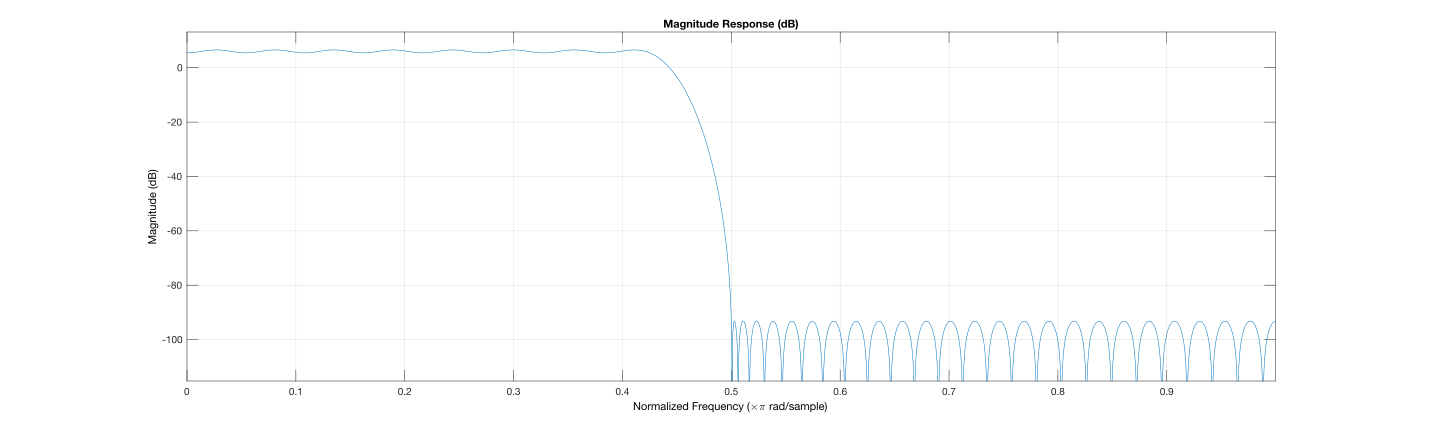
\includegraphics[height = 0.5\textwidth, width = 1.2\textwidth]{PM_direct.pdf}
		\caption{Parks-McClellan Filter}
		\label{mgpm}
	\end{subfigure}
	\hfill
	\begin{subfigure}[b]{0.5\textwidth}
		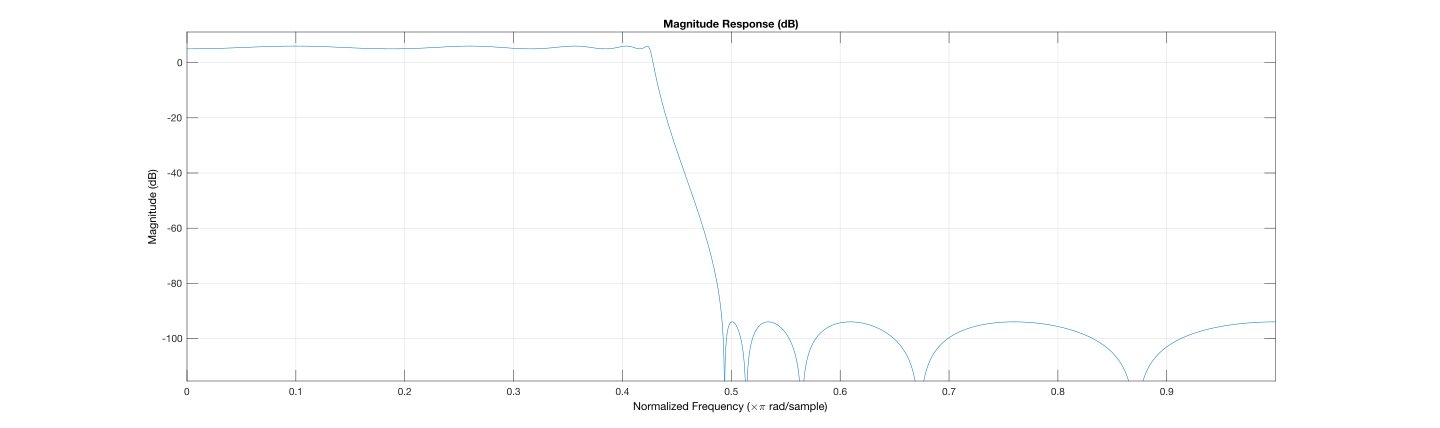
\includegraphics[height = 0.5\textwidth, width = 1.2\textwidth]{Ellip_direct.pdf}
		\caption{Elliptic Filter}
		\label{mgellip}
	\end{subfigure}
	\caption{Magnitude Responses}\label{Figure 3.6}
\end{figure}

\newpage

The filter have been designed in \MATLAB. The common procedure \cite{matlab} requires to specify the normalizing frequency (to transition from continuous to digital frequency). Hereunder, it is the normalizing frequency after the upsampling block $L$ which we call:

\begin{align}
	F_e = LFs_{in} \label{eqn:Fmax}
\end{align}
 
\subsubsection{Efficiency}

As well as a conversion of high quality with no aliasing or any other artifacts, an efficient filter, that processes data rapidly is desired. The decision was made that what undoubtedly counts is how many multiplications will be necessary to generate a single sample at the output. In this way, we define the number of \textit{Multiplications Per Output Samples} or MPOS. The lower it is, the lower the computation requirements will be, which is what we need for a real-time process. In the case of a direct implementation of a \hyperlink{FIR}{FIR} or  \hyperlink{IIR}{IIR} filter of order $N$, we have:

\begin{align}
	MPOS = (N + 1)M \label{eqn:mpos_direct} 
\end{align} 

It is conspicuous that if the length of the filter (i.e. the  number of its coefficients) is too considerable, the number of MPOS will enlarge resulting in an extremely slow transformation \footnote{This is particularly true for a direct implementation of FIR filters because the order is larger than IIR filters. However, we can still improve the efficiency for the IIR case, even if it appears to be already good.}. Thus, the need for improvement would be clearly an obligation.
\subsection{Improvements} 

In many cases, the numbers $L$ and $M$ are actually too large, making the computation of the filter's coefficients unfeasible (especially for the FIR case; cf. table \ref{tab:filters}). For example, with a conversion from 44.1 kHz to 48 kHz, the resampling factor is then $\frac{L}{M} = \frac{160}{147}$. For a direct implementation, the order of the filter will be high, making the computation of the coefficients unstable. A well known method to address this issue is the polyphase decomposition which permits a more efficient implementation of a given transfer function. Moreover, the decomposition into several cascaded stages is also explored in this section.


\subsubsection{Polyphase}

The polyphase decomposition is a different way to express the impulse response of the filter. Instead of convolving the signal by the whole filter's \hyperlink{IR}{IR}, only parts of this response are used and they process the input signal simultaneously.
 It is a parallel representation that can considerably reduce the amount of complexity needed to perform a sampling rate conversion. 

The classic method \cite{Oppenheim}, \cite{oppenheim2} would be to decompose the filter's impulse response $h[n]$ into M (or L) subsequences $h_k[n]$ with $ k = 0, 1, \dots, M-1$ such as


\begin{align}
h_k[n] = 
	\begin{cases}
	h[n + k], & \quad n \,\text{= integer multiple of} \,M, \\ 
	0, & \quad \text{otherwise}. \label{eqn:subsequences}
	\end{cases}
\end{align}

Now, if we consider the z-transform of the impulse response of the filter,

\begin{align}
	H(z) = \sum\limits_{n=-\infty}^{\infty} h[n]z^{-n} \label{eqn:ztrans}
\end{align}

we can rewrite it in the following form

	\begin{align} \label{eqn:ztranspoly}
		H(z) &= \sum\limits_{n=-\infty}^{\infty} h[nM]z^{-nM} \nonumber\\ 
		&+ z^{-1} \sum\limits_{n=-\infty}^{\infty} h[nM+1]z^{-nM} \\ 
		&\vdots \nonumber \\*
		&+ z^{-(M-1)} \sum\limits_{n=-\infty}^{\infty} h[nM+M-1]z^{-nM} \nonumber 
	\end{align}

This can be compactly written as 

\begin{align}
H(z) = \sum\limits_{k=0}^{M-1} E_k(z^M)z^{-k} \label{eqn:compact}
\end{align}

where

\begin{align}
E_k(z) = \sum\limits_{n=-\infty}^{\infty} e_k[n]z^{-n} \label{eqn:zpolycomp}
\end{align}

with

\begin{align}
e_k[n] = h[nM + k], \quad 0 \leq k \leq M-1 \label{eqn:polycomp}
\end{align}

The $E_k(z)$ are called the \textit{polyphase components} of $H(z)$, obtained by z-transform \cite{Oppenheim} of the $e_k[n]$. Equation \ref{eqn:compact} is referenced as type 1 polyphase \cite{vaidyanathan}. An alternative notation can also be presented, named type 2 polyphase:

\begin{align}
	H(z) = \sum\limits_{k=0}^{M-1} R_k(z^M)z^{-(M-1-k)} \label{eqn:poly2}
\end{align}

where the components $R_k(z)$ are simply a permutation of the $E_k(z)$ i.e. $R_k(z) = E_{M-1-k}(z)$.\\ 

According to this notation, we are now able to present a classic representation of a polyphase implementation of a sample-rate conversion system displayed underneath in figure \ref{Figure 3.7}.


\begin{figure}[htb!]
	\centering
	\begin{subfigure}[b]{\textwidth}
		\centering
		\includegraphics[scale=0.95]{polyphase_direct_M.pdf}
		\vspace*{1mm}
		\caption{Direct Implementation of Type 1 Polyphase}\label{3.7.a}
	\end{subfigure}	
\end{figure}



\begin{figure}[htb!] %\ContinuedFloat
	\centering
	\begin{subfigure}[b]{\textwidth}
		\centering
		%\hbox{\hspace{2em} 
		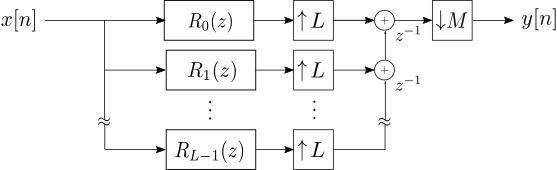
\includegraphics[scale=0.95]{polyphase_direct_L.pdf}%}
		\vspace*{1mm}
		\caption{Direct Implementation of Type 2 Polyphase}\label{3.7.b}
	\end{subfigure}	
	\caption{Classic Polyphase Decomposition for \protect\hyperlink{SRC}{SRC} Systems}
	\label{Figure 3.7}
\end{figure}

At this point, the reader might wonder why the block $M$ in figure \ref{3.7.a} or the $L$ one in Figure \ref{3.7.b} are placed respectively before and after the polyphase components. This has been made possible thanks to the \textit{Noble Identity} introduced in \cite[p.~204-205]{Oppenheim}.

These structures considerably reduce the amount of MPOS required for the computation since currently with have $MPOS = \frac{(N+1)M}{M} = (N+1)$ for the type 1 polyphase and $MPOS = \frac{(N+1)M}{L} $ for the type 2 polyphase. However, these arrangements are not the most efficient ones since the polyphase components are not applied at the lowest rate where the hardware complexity is the lowest. This is due to the fact that the expander $L$ and the decimator $M$ are not interchangeable (we cannot apply the noble identity again). Nonetheless, the next section describes what solution has been retained to further enhance our procedure.

\newpage

\paragraph{Polyphase Representation for FIR Filters}
\justify

Before we proceed, it is important to specify that the above polyphase decompositions can only be implemented to a non-recursive filter, that is a filter that only uses the input values to compute its coefficients. Typically, these filters are referred as \hyperlink{FIR}{FIR} filters. 

For the purpose of having an efficient polyphase structure, as explained in \cite{vaidyanathan}, we can exploit the fact that the  $k^{th}$ polyphase term in equation \ref{eqn:compact} can be substituted by $z^{-Lka}z^{Mkb}$ with $a$ and $b$ positive integers. As long as $L$ and $M$ are relatively prime (common divisor is 1), the terms $a$ and $b$ can be found according to the Euclid's Theorem since we have $La-Mb=1$. As of now, every delay $z^{-1}$ in figure \ref{Figure 3.7} can be replaced by $z^{-La}z^{Mb}$, thus the expander and decimator can be interchanged which leads to the following structure displayed on the next page (figure \ref{Figure 3.8}).

\begin{figure}[ht!]
	\centering
	\includegraphics[scale=0.95]{polyphase_direct_efficient.pdf}
	\vspace*{1mm}
	\caption{Efficient Polyphase Decomposition}
	\label{Figure 3.8}
\end{figure}



Thanks to this final representation, the \hyperlink{MPOS}{MPOS} is now decreased:

\begin{align}
	MPOS =  \frac{(N+1)M}{LM} = \frac{(N+1)}{L}\label{eqn:final_poly}
\end{align}

As a result, we obviously chose to use this decomposition. The integers $a$ and $b$ are simply pre-computed in accordance with the values of $L$ and $M$ by means of the \textit{Euclidean Algorithm}.


\paragraph{Polyphase Representation for IIR Filters}

\justify

For the \hyperlink{IIR}{IIR} filters, the trick is a little bit more complex. As previously described, the former polyphase decomposition can only be applied to a non-recursive filter. Nevertheless, IIR filters are composed of both a recursive and a non-recursive part. Let us take a closer look at its transfer function given by 

\begin{align}
	H(z) = \frac{B(z)}{A(z)} =  \frac{\sum\limits_{k=0}^{N_z} b_kz^{-k} }{\sum\limits_{k=0}^{N_p} a_kz^{-k}}
	\label{eqn:3.14}
\end{align}

where $N_z$ and $N_p$ are the number of zeros and poles respectively. As we can see, the numerator represents the non-recursive part and the denominator the recursive one. The main goal here is to be able to use the polyphase decomposition presented in figure \ref{Figure 3.8}. To do so, we need to isolate the non-recursive part. A straightforward approach would be to simply move the numerator $B(z)$ before the expander $L$ such as illustrated in the figure below.

\begin{figure}[ht!]
	\centering
	\includegraphics[scale=0.8]{iir_direct_poly.pdf}
	\caption{Direct Polyphase Implementation for IIR Filter}
	\label{Figure 3.9}
\end{figure}

By doing this, the polyphase decomposition can be applied upon the polynomial $B(z^{\frac{1}{L}})$ where the working sampling frequency is lower than at its former position, meaning the complexity is lessened:

%\begin{align}
%	MPOS = (\textcolor{blue}{\frac{N+1}{L}} + \textcolor{orange}{N} + \textcolor{cyan}{1})* M
%\end{align}
%
%The term in blue comes from the polyphase separation, the one in orange from the coeffients of $A(z)$ and the last cyan term take into account the gain of the overall filter.   

\begin{align}
	MPOS = (\frac{N_z+1}{L}\ + N_p + 1)M\label{eqn:3.15}
\end{align}

Nevertheless, this structure is not the most efficient one since, as before, not all the blocks have been dealt with, that is to say, $A(z)$. An improvement is still possible.\\

Since $H(z)$ is a fraction of two polynomials, we can factorize them and then rewrite the transfer function in the following way

\begin{align}
	H(z) = k\frac{\prod\limits_{k=1}^{N_z} (1 - z_k z^{-1} )}{\prod\limits_{k=1}^{N_p} (1 - p_k z^{-1})}
	\label{eqn:3.16}
\end{align}

with $z_k$ the \textit{zeros}, $p_k$ the \textit{poles} and $k$ the gain. At present, we can have recourse to the substitution 

\begin{align}
	1 - p_kz^{-1} \equiv \frac{1 - p_k^Dz^{-D}}{\sum\limits_{i=0}^{D-1}p_k^iz^{-i}}
	\label{eqn:3.17}
\end{align} 


The next step is to replace equation \ref{eqn:3.17} in \ref{eqn:3.16} but we need to assign some values to $D$. The point is to split the poles and raise them to the power of $L$ and $M$ to then be able to use the noble identity. To make it clearer, let's say we have $N_z$ poles and we arbitrarily choose two values $N_L$ and $N_M$ such as $N_L + N_M = N_z$. Now we pick $N_L$ poles $\gamma$ among the $p_k$ with $D = L$ and the $N_M$ $\epsilon$ remaining with $D = M$. The poles we select do not matter, the only important rule to fulfill is to not separate the complex conjugate poles. 

Therefore, we can expand equation \ref{eqn:3.16}

\begin{equation}
	\begin{aligned}
H(z) &= k\cfrac{\prod\limits_{k=1}^{N_z} (1 - z_k z^{-1} )}{\prod\limits_{k=1}^{N_L} (1 - \gamma_k z^{-1})\prod\limits_{k=1}^{N_M} (1 - \epsilon_k z^{-1})} \\ 
&= \cfrac{k\prod\limits_{k=1}^{N_z} (1 - z_k z^{-1} )}{\prod\limits_{k=1}^{N_L} \cfrac{1 - \gamma_k^L z^{-L}}{\sum\limits_{i=0}^{L-1}\gamma_k^i z^{-i}} \prod\limits_{k=1}^{N_M} \cfrac{1 - \epsilon_k^M z^{-M}}{\sum\limits_{i=0}^{M-1}\epsilon_k^i z^{-i}}} \\
& = \cfrac{k\prod\limits_{k=1}^{N_z} (1 - z_k z^{-1} ) \prod\limits_{k=1}^{N_L}\Big (\sum\limits_{i=0}^{L-1}\gamma_k^i z^{-i} \Big )\prod\limits_{k=1}^{N_M} \Big (\sum\limits_{i=0}^{M-1}\epsilon_k^i z^{-i} \Big )}{\prod\limits_{k=1}^{N_L} (1 - \gamma_k^L z^{-L}) \prod\limits_{k=1}^{N_M} (1 - \epsilon_k^M z^{-M}) }
\label{eqn:3.18}
	\end{aligned}
\end{equation}

To simplify the numerator, we can return to the first definition of $H(z)$ (cf. equation \ref{eqn:3.14}) and rewrite $k\prod\limits_{k=1}^{N_z} (1 - z_k z^{-1})$ as $\sum\limits_{k=0}^{N_z} b_kz^{-k}$.
Then, for the two other products we have to recall that it is a multiplication of polynomials. In other words, if we consider first the product over $N_L$, it is a multiplication of polynomials of coefficients $\Gamma_k = [\gamma_k^0, \gamma_k^1, \dots, \gamma_k^{L-1}] \;for\; k = 1, \dots, N_L$. Thereby, if we name $cL$ the list of coefficients of this product, we end up with $cL = \Gamma_1*\dots*\Gamma_{N_L-2}*\Gamma_{N_L-1}*\Gamma_{N_L}$where $*$ designates the \textit{linear convolution}. 

All this leads to 

\begin{align}
	\prod\limits_{k=1}^{N_L}\Big (\sum\limits_{i=0}^{L-1}\gamma_k^i z^{-i} \Big ) = \sum\limits_{i=0}^{N_L(L-1)}cL_i\,z^{-i}
	\label{eqn:3.19}
\end{align}

where $cL_i$ represents the $i^{\text{th}}$ coefficient of the list $cL$. Likewise

\begin{align}
\prod\limits_{k=1}^{N_M}\Big (\sum\limits_{i=0}^{M-1}\epsilon_k^i z^{-i} \Big ) = \sum\limits_{i=0}^{N_M(M-1)}cM_i\,z^{-i}
\label{eqn:3.20}
\end{align}

Finally, the transfer function takes the form of 

\begin{align}
	H(z) = \cfrac{\sum\limits_{k=0}^{N_z} b_kz^{-k}\sum\limits_{i=0}^{N_L(L-1)}cL_i\,z^{-i}\sum\limits_{i=0}^{N_M(M-1)}cM_i\,z^{-i}}{\prod\limits_{k=1}^{N_L} (1 - \gamma_k^L z^{-L}) \prod\limits_{k=1}^{N_M} (1 - \epsilon_k^M z^{-M})}
\end{align}

Anew, this last equation is the product of three polynomials. It simply gives 

\begin{align}
H(z) = \cfrac{\sum\limits_{k=0}^{N_N} c_kz^{-k}}{\prod\limits_{k=1}^{N_L} (1 - \gamma_k^L z^{-L}) \prod\limits_{k=1}^{N_M} (1 - \epsilon_k^M z^{-M})} = \cfrac{H_N(z)}{H_L(z^L)H_M(z^M)}\label{eqn:3.22}
\end{align}

with $N_N = N_z + N_L(L-1) + N_M(M-1)$ and $c = b*cL*cM$. \\


The final expression of $H(z)$ is composed of three filters: 

\begin{enumerate}
	\item $H_N(z) = \sum\limits_{k=0}^{N_N} c_kz^{-k}$ which is \hyperlink{FIR}{FIR};
	\item $H_L(z^L)  = \cfrac{1}{\prod\limits_{k=1}^{N_L} (1 - \gamma_k^L z^{-L})}$, an all-pole filter, function of $z^L$;
	\item $H_M(z^M) = \cfrac{1}{\prod\limits_{k=1}^{N_M} (1 - \epsilon_k^M z^{-M})}$ which is also an all-pole filter, function of $z^M$.
\end{enumerate}

\newpage
The structure of the sampling rate conversion is henceforward

\begin{figure}[ht!]
	\centering
	\hspace*{-5mm}
	\includegraphics[scale = 0.8]{russell.pdf}
	\caption{Decomposition of $H(z)$ as a Cascaded Structure}
	\label{Figure 3.10}
\end{figure}

As depicted in the above figure, the procedure formerly detailed has introduced two filters $H_L(z^L)$ and $H_M(z^M)$ that can be moved respectively accross the expander and the decimator thanks to the noble identity. Furthermore, we can perform the polyphase decomposition seen in figure \ref{Figure 3.8} on $H_N(z)$ since it is a FIR filter. It follows

\begin{figure}[ht!]
	\centering
	\includegraphics[scale = 0.7]{russell_final.pdf}
	\caption{Efficient Implementation of an IIR Filter for a \protect\hyperlink{SRC}{SRC}}
	\label{Figure 3.11}
\end{figure}


This final arrangement is an efficient implementation for IIR filters. It has been introduced in \cite{russell}. Although the numerator order is increased by $N_L(L-1) + N_M(M-1)$, the gain in efficiency over the direct implementation is $LM$ for the numerator and $LM/(L+M-1)$ with a number of \hyperlink{MPOS}{MPOS} of

\begin{equation}
	\begin{aligned}
	MPOS &= N_M + \frac{1}{L} (N_N+1) + \frac{M}{L} N_L \\
	&= \frac{1}{L} (N_z +1) + \frac{L+M-1}{L} N_p 
	\label{eqn:3.23}
	\end{aligned}
\end{equation}

It appears from this last equation that the number of MPOS does not depend on $N_M$ or $N_L$, therefore, we can just as well set one of these factors to zero. This method should be prefered over using a FIR filter since the efficiency is greatly enhanced. 


\subsubsection{Multistage}\label{3.1.4.2}

Even so, another improvement is still possible. It is based on dividing the factors $L$ and $M$ into $N$ factors i.e. $L = \prod_{i=1}^{N}L_i$ and $M=\prod_{i=1}^{N}M_i$ where some $L_i$ and $M_i$ can be equal to $1$ but are relatively prime $\forall \,  i,j$. The goal is to cascade the stages $L_i$ and $M_i$ and compute every filter $H_i$ (cf. figure \ref{Figure 3.12}). By doing so, the orders are drastically lowered and so are the \hyperlink{MPOS}{MPOS}. 

\begin{figure}[ht!]
	\centering
	\includegraphics[scale = 0.7]{multistage.pdf}
	\caption{Multistage Representation}
	\label{Figure 3.12}
\end{figure}

\newpage
The overall filter can be found again by applying multiple noble identities

\begin{align}
	H(z) = 	\prod_{i=1}^{N} H_i(z^{\tilde{L}_i \tilde{M}_{i-1}})
	\label{eqn:3.24}
\end{align}

With the notation $\tilde{L}_i$ and $\tilde{M}_{i}$ standing for $\prod_{k=i+1}^{N}L_k$ and $\prod_{k=1}^{i}M_k$ respectively and $\tilde{L}_N = \tilde{M_0} = 1$.\\


This approach called \textit{multistage} has been widely utilized in interpolators and decimators \cite{Proakis}, \cite{Oppenheim}, \cite{vaidyanathan}, \cite{turek}. It allows less constraints on the filters by reducing their orders and therefore the MPOS is lower than a direct implementation

\begin{equation}
	MPOS = (N_1 + 1)M_1 \frac{L_2}{M_2}\dots\frac{L_N}{M_N} + (N_2 + 1)M_2 \frac{L_3}{M_3}\dots \frac{L_N}{M_N} + \dots (N_N + 1)M_N 
	\label{eqn:3.25}
\end{equation}

with $N_i$ the order of the filter $i$.\\

For the case of sample-rate conversion by a fractional factor, two methods on how to design the filters have been investigated in this project:

\begin{itemize}
	\item The first one may be called the \textit{classic} one. It follows the same theory behind a one-stage system as seen in section \ref{section 3.1.3}. The difference here resides in the calculation of the cutoff frequencies. For each stage $i$
	\begin{align}
		\omega_{c_i} = min\Big(\frac{\pi}{L_i},\frac{\pi}{M_i}\Big), \quad i = 1,2,\dots N. \label{eqn:3.26}
	\end{align}
	and,
	\begin{align}
		H_i(1) = L_i, \quad i = 1,2,\dots N. \label{eqn:3.27}
	\end{align}
	 	
	 \item The second method has been introduced by \textit{Crochiere} and \textit{Rabiner} in \cite{crochiere} (we will reference it as \textit{second method}). We decided to explore this solution because \textit{Smarc}, an open source project by \textit{Télécom ParisTech} \cite{paristech} chose this process with \hyperlink{FIR}{FIR} Parks-McClellan filters implemented in polyphase decomposition and it gave decent results (cf \ref{section 3.2.6}). To explain the manner to process, we can defferentiate two cases:
	 
	 \begin{enumerate}
	 	\item $L/M < 1$
	 	
	 	Let's consider the first case when $L/M$ is $<1$ that is identified as a decimator. The way to proceed is to separate the system into several blocks $D_K$ depicted in the figure \ref{Figure 3.13} with 
	 	
	 	\begin{align}
	 		D_i = \frac{M_i}{L_i} > 1, \quad i = 1,2,\dots K.\label{eqn:3.28}
	 	\end{align} 
	 	
	 	and,
	 	\begin{align}
	 		f_{ri} = \frac{f_{r(i-1)}}{D_i} = \frac{L_i}{M_i}f_{r(i-1)}, \quad i = 1,2,\dots K.
	 	\end{align}
	 	
	 	\begin{figure}[ht!]
	 		\centering
	 		\hspace*{10mm}
	 		\includegraphics[scale = 0.68]{multistage_sup1_1.pdf}
	 		\caption{Representation of K-stage Decimator}\label{Figure 3.13}
	 	\end{figure}
 	
 	The initial sampling rate is $f_{r0}$ and the final one is $f_{rK}$ with  $f_{r0} > f_{rK}$. The global reduction factor is $D = \frac{f_{r0}}{f_{rK}} = \prod_{i=1}^{K} D_i$, greater than $1$. A block $D_i$ is equivalent to a stage $i$ presented in figure \ref{Figure 3.12}, the difference lies in the design of the filters: the stopband of the filters has to be adapted for each stage without modifying the passband. The way to do so is sketched as follows\\
 	
 	\begin{figure}[ht!]
 		\centering
 		\hspace*{15mm}
 		\includegraphics[scale = 1]{multistage_sup1_2.pdf}
 		\caption{Frequency Response Interpretation of the \\K-stage Decimation Process}\label{Figure 3.14}
 	\end{figure}
 
 $f_s$ is the maximal frequency in the signal through each stage 
 
 \begin{align}
 	fs \leq \frac{F_{rK}}{2}
 \end{align}
 It can be noticed that the passband never changes but the stopband is. However the equivalent digital passband frequency $\omega_{p_i} = f_p/f_{ri}$ is different for every stage. A thorough method to find the most optimized $D_i$ has been demonstrated in \cite{crochiere} for a chosen number of stage $K$. Nevertheless, it depends on abacuses and always result in approximating their values since they need to be integers. What has been shown in \cite{turek} is the importance of the number of stages on the overall efficiency: for $K = 3$ or $4$, the MPOS is the lowest. Having this in mind, the values of $L_i$ and $M_i$ for a given ratio $L/M$ with this amount of stages are often unique. Thus, it may not be worthwhile to use this tedious method of choosing the $D_i$, but simply pick them manually, especially if we choose a high number of stages.\\
 	
 
	 	\item $L/M > 1$
	 	
	 	For the case of $L/M > 1$ that is, the case of interpolation, the reasoning is the same. This time
	 	
	 	\begin{align}
	 		f_{r(i-1)} = D_i f_{ri} , \quad i = 1,2,\dots K.
	 	\end{align}
	 	
	 	with  $D_i = \frac{M_i}{L_i} > 1$ (the role of $M_i$ and $L_i$ are reversed). Since interpolation is the dual of decimation, we have 
	 	
	 	\begin{figure}[ht!]
	 		\centering
	 		%\hspace*{15mm}
	 		\includegraphics[scale = 0.6]{multistage_down_1.pdf}
	 		\caption{Representation of K-stage Interpolator}\label{Figure 3.15}
	 	\end{figure}
	 	
	 	and the filter design in the frequency domain
	 	
	 	\begin{figure}[ht!]
	 		\centering
	 		\hspace*{2mm}
	 		\includegraphics[scale = 0.77]{multistage_down_2.pdf}
	 		\caption{Frequency Response Interpretation of the \\ K-stage Interpolation Process}\label{Figure 3.16}
	 	\end{figure}
	 	
	 	The same comment made in regard to how to find the $D_i$ applies here.\\
	 	Although these two methods are different design-wise, they share a common feature. The passband ripple has to be altered for both cases. If we desire the total passband (after combination of all the stage filters) to be the same as chosen originally by the filter specifications, we must now have $R_p = \frac{R_p}{\text{Number of Stages}}$. However, the stopband attenuation remains unchanged (see \cite{Proakis}). Moreover, equation \ref{eqn:3.27} is still valid for this approach. 
	 	In conclusion, what remains is comparing these two methods and discover which one gives best quality and efficiency result (\hyperlink{MPOS}{MPOS}).
	 	
	 \end{enumerate}
	 
\end{itemize}

One could wonder what the influence of the organization of the stages is, in other words, which $L_i$ and $M_i$ are best for which stage. But let us present an example to buttress our concern.

In this example, we consider the case where $L=9$, $M=8$ and a number of stages $N=2$. Since, 
$L_1=L_2=3$, the result is two possible implementations of a dual stage \hyperlink{SRC}{SRC}.


\begin{itemize}

\item \textbf{Case $M_1=2$ and $M_2=4$} \label{example1}

%\begin{center}
%	\begin{tikzpicture}
%	\node[dspnodeopen,dsp/label=above] (e0) {$F_\text{sin}$};
%	\node[dspsquare,right=of e0] (e1) {$\upsamplertext{3}$};
%	\node[dspfilter,right=of e1,xshift=-.3cm,minimum width=1cm] (e2) {$H_1$};
%	\node[dspsquare,right=of e2,xshift=-.3cm] (e3) {$\downsamplertext{2}$};
%	\node[dspsquare,right=of e3,xshift=-.3cm] (e4) {$\upsamplertext{3}$};
%	\node[dspfilter,right=of e4,xshift=-.3cm,minimum width=1cm] (e5) {$H_2$};
%	\node[dspsquare,right=of e5,xshift=-.3cm] (e6) {$\downsamplertext{4}$};
%	\node[dspnodeopen,right=of e6,dsp/label=above] (e7) 
%	{$F_\text{sout}$};
%	\foreach \i [evaluate=\i as \j using int(\i+1)] in {0,1,...,6} {
%		\draw[dspconn] (e\i) -- (e\j);
%	}
%	\end{tikzpicture}
%\end{center}

\begin{figure}[ht!]
	\centering
	\includegraphics[scale=0.8]{multistage_ex_1.pdf}
	\caption{Corresponding 2-stage decomposition}\label{Figure 3.17}
\end{figure}

The cutoff frequencies of $H_1$ and $H_2$ are $\pi/3$ and $\pi/4$, respectively.
We have $H(z)=H_1(z^3)H_2(z^2)$. As the following plot shows, there should be 
no problem :
\begin{itemize}
	\item outside of low frequencies, the filters act on different 
	frequency bands,
	\item the resulting cutoff pulsation is $\pi/9$ as expected.
\end{itemize}


\begin{figure}[h]
\centering
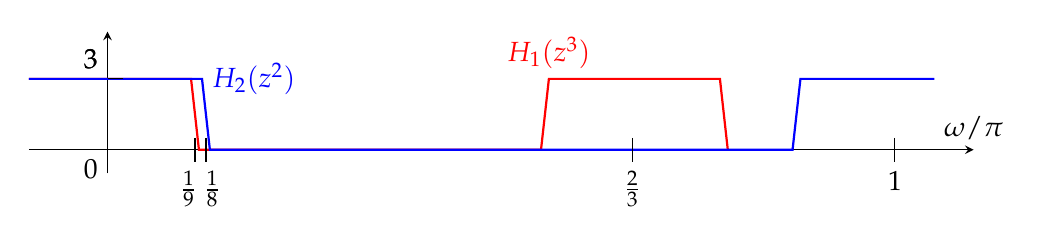
\begin{tikzpicture}[>=stealth,x=10cm,y=3mm]
	\draw[->] (-.1,0)--(1.1,0) node[above]{$\omega/\pi$};
	\draw[->] (0,-1)--(0,5);
	\draw[red,thick] (-.1,3)--({1/9-.005},3) 
	--++(.01,-3)--({5/9-.005},0)--++(0.01,3)node[above]{$H_1(z^3)$}--++({2/9-.005},0)--++(.01,-3););
	\draw[blue,thick] 
	(-.1,3)--({1/8-.005},3)node[right]{$H_2(z^2)$}--++(.01,-3)--({7/8-.005},0) 
	--++(0.01,3)--(1.05,3);
	\draw (1/9,.5)--++(0,-1) node[below, xshift=-0.08cm] {$\frac{1}{9}$};
	\draw (1/8,.5)--++(0,-1) node[below, xshift=0.08cm] {$\frac{1}{8}$};
	\draw (2/3,.5)--++(0,-1) node[below] {$\frac{2}{3}$};
	\draw (1,.5)--++(0,-1) node[below] {$1$};
	\draw (.02,3)--++(-.02,0) node[above left] {$3$};
	\draw (.02,3)--++(-.02,0) node[above left] {$3$};
	\node[below left] at (0,0) {$0$};
\end{tikzpicture}
\caption{Frequency Representation of Resulting Filters}\label{Figure 3.19}
\end{figure}


\item \textbf{Case $M_1=4$ and $M_2=2$} \label{example2}


%\begin{center}
%	\begin{tikzpicture}
%	\node[dspnodeopen,dsp/label=above] (e0) {$F_\text{in}$};
%	\node[dspsquare,right=of e0] (e1) {$\upsamplertext{3}$};
%	\node[dspfilter,right=of e1,xshift=-.3cm,minimum width=1cm] (e2) {$H_1$};
%	\node[dspsquare,right=of e2,xshift=-.3cm] (e3) {$\downsamplertext{4}$};
%	\node[dspsquare,right=of e3,xshift=-.3cm] (e4) {$\upsamplertext{3}$};
%	\node[dspfilter,right=of e4,xshift=-.3cm,minimum width=1cm] (e5) {$H_2$};
%	\node[dspsquare,right=of e5,xshift=-.3cm] (e6) {$\downsamplertext{2}$};
%	\node[dspnodeopen,right=of e6,dsp/label=above] (e7) 
%	{$F_\text{out}$};
%	\foreach \i [evaluate=\i as \j using int(\i+1)] in {0,1,...,6} {
%		\draw[dspconn] (e\i) -- (e\j);
%	}
%	\end{tikzpicture}
%\end{center}

\begin{figure}[ht!]
	\centering
	\includegraphics[scale=0.8]{multistage_ex_2.pdf}
	\caption{Corresponding 2-stage decomposition}\label{Figure 3.18}
\end{figure}

The cutoff frequencies of $H_1$ and $H_2$ are $\pi/4$ and $\pi/3$, respectively.
We have $H(z)=H_1(z^3)H_2(z^4)$. As the following plot shows, the situation is 
now more complicated because
\begin{itemize}
	\item the filters share common frequency intervals in 
	high frequencies,
	\item the resulting cutoff pulsation of $\pi/12$ is lower than expected.
\end{itemize}



\begin{figure}[ht!]
	\centering
	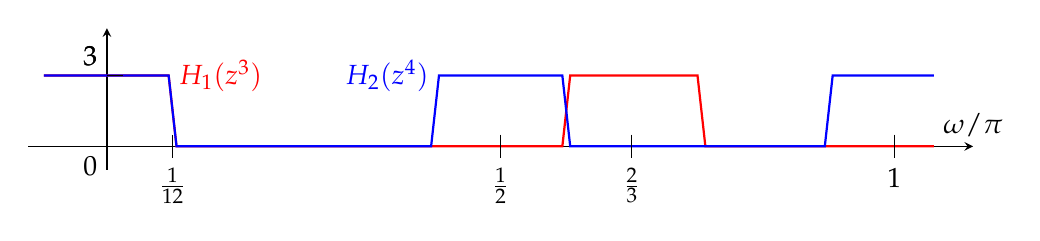
\begin{tikzpicture}[>=stealth,x=10cm,y=3mm]
	\draw[->] (-.1,0)--(1.1,0) node[above]{$\omega/\pi$};
	\draw[->] (0,-1)--(0,5);
	\draw[red,thick] (-.08,3)--({1/12-.005},3) node[right]{$H_1(z^3)$}
	--++(.01,-3)--({7/12-.005},0)--++(0.01,3)--++({1/6-.005},0)--++(.01,-3)--(1.05,0);
	\draw[blue,thick] (-.08,3)--({1/12-.005},3)--++(.01,-3)--({5/12-.005},0)
	--++(0.01,3)node[left]{$H_2(z^4)$} 
	--({7/12-.005},3)--++(0.01,-3)--({11/12-.005},0)--++(.01,3)--(1.05,3);
	\draw (1/12,.5)--++(0,-1) node[below] {$\frac{1}{12}$};
	\draw (1/2,.5)--++(0,-1) node[below] {$\frac{1}{2}$};
	\draw (2/3,.5)--++(0,-1) node[below] {$\frac{2}{3}$};
	\draw (1,.5)--++(0,-1) node[below] {$1$};
	\draw (.02,3)--++(-.02,0) node[above left] {$3$};
	\draw (.02,3)--++(-.02,0) node[above left] {$3$};
	\node[below left] at (0,0) {$0$};
	\end{tikzpicture}
	\caption{Frequency Representation of Resulting Filters}\label{Figure 3.20}
\end{figure}


What can be retained from this example is that if the first stage is composed of the factors $L_1$ and  $M_1$ such that $M_1 > L_1$, this will result in a degradation of the signal. More generally, we can extract two rules out of these examples:
\begin{itemize}\label{3.1.4.2.conclusion}
	\item[--] if $L > M$ ($F_{s_{out}} > F_{s_{in}}$), to avoid alisasing, every intermediary frequencies $F_{int}$ must not be smaller than $F_{s_{in}}$.
	\item[--] if $M > L$ ($F_{s_{in}} > F_{s_{out}}$), $F_{int}$ must not be smaller than $F_{sout}$ to avoid alisasing. 
\end{itemize}
The section \ref{section 3.2.2} will delve into how properly organize the stages while considering the above aspect. 



\subsubsection{Multistage and Polyphase}

Just as polyphase, multistage decomposition can improve how to decrease the number of Multiplications Per Output Sample which is crucial if we want to process data in real-time. Evidently, we can combine these advancements. 

\begin{itemize}
	\item For \hyperlink{FIR}{FIR} filters, the final structure would be a combination of figures \ref{Figure 3.12} and \ref{Figure 3.8} for evey stage $i$. Moreover we can use the property that these filters can be implemented as a symetric structure called \textit{folded structure} which will divide the direct \hyperlink{MPOS}{MPOS} (cf. equation \ref{eqn:mpos_direct}) by 2. Thus, the final number of multiplications is 
	
	\begin{align}
		MPOS = \frac{(N_1 + 1)M_1}{2L_1} \frac{L_2}{M_2}\dots\frac{L_N}{M_N} + \frac{(N_2 + 1)M_2}{2L_2} \frac{L_3}{M_3}\dots \frac{L_N}{M_N} + \dots +\frac{(N_N + 1)M_N}{2L_N} 
		\label{eqn:3.32}
	\end{align}
	\item For \hyperlink{IIR}{IIR} filters, the final structure would be a combination of figures \ref{Figure 3.12} and \ref{Figure 3.11} for evey stage $i$. Therefore, we have
	
	\begin{align}\label{eqn:3.33}
	MPOS =& \Big (\frac{1}{L_1} (N_{z_1} +1) + \frac{L_1+M_1-1}{L_1} N_{p_1} \Big ) \frac{L_2}{M_2}\dots\frac{L_N}{M_N} +  \nonumber\\ 
	&\Big (\frac{1}{L_2} (N_{z_2} +1) + \frac{L_2+M_2-1}{L_2} N_{p_2} \Big ) \frac{L_3}{M_3}\dots \frac{L_N}{M_N} + \\\nonumber
	&\dots +\Big (\frac{1}{L_N} (N_{z_N} +1) + \frac{L_N+M_N-1}{L_N} N_{p_N} \Big ) 
	\end{align}
	
	In this case, if we apply the same folded structure principle  to the resulting FIR part $H_N(z)$ in equation \ref{eqn:3.22}, the number of MPOS would depend on $N_M$ and $N_L$ since
	
	 
\end{itemize}


\end{itemize}

\newpage

\begin{small}

\begin{align}
MPOS = &\Bigg (\frac{ (N_{z_1} +1) }{2L_1}+ \frac{N_{M_1}(2L_1+M_1-1)+N_{L_1}(2M_1+L_1-1)}{2L_1}  \Bigg ) \frac{L_2}{M_2}\dots\frac{L_N}{M_N} + \nonumber\\ 
&\Bigg (\frac{ (N_{z_2} +1)}{2L_2} + \frac{N_{M_2}(2L_2+M_2-1)+N_{L_2}(2M_2+L_2-1)}{2L_2} \Bigg ) \frac{L_3}{M_3}\dots \frac{L_N}{M_N} +\nonumber\\
&\vdots \nonumber\\ 
&+\Bigg (\frac{ (N_{z_N} +1)}{2L_N} + \frac{N_{M_N}(2L_N+M_N-1)+N_{L_N}(2M_N+L_N-1)}{2L_N} \Bigg) 
\end{align}

\end{small}
Minimizing this last equation might be more difficult than minimizing equation \ref{eqn:3.33}. Thus, the latter should be the one to consider. 

\subsection{Conclusion}


The common methods to realize a sample-rate conversion by a rational factor $L/M$ have been studied through this part. The classical principle would be to select an expander $L$, a low-pass filter and a decimator $M$. Multiple filters could be used and usually FIR ones because of their linear phase. Nevertheless, the choice has been made to utilize a FIR Parks-McClellan filter and an IIR Elliptic one to compare the  quality of the conversion and their efficiency in terms of MPOS. Some improvements have to be considered such as polyphase and multistage decompositions if real-time performance is required. The next part will now focus on a real case: implementing and comparing the previous statements  in order to confirm or disconfirm them. 

%\newpage

\section{Study Case}

In this section, we will apply the theory described earlier to a tangible example. We decided to study the case of converting from 44.1 kHz to 48 kHz and vice versa. The methods explained in this part are applicable to any rational sampling rate conversion ratio. However, for illustration and practical purposes, we will focus on this particular case.

\subsection{Filter Specifications}\label{section 3.2.1}
As already stated, this conversion requires a ratio of $160$ over $147$ and if we use filters with low error tolerances (with regard to an ideal lowpass filter), the order is in general high thus imposing increasing the computational complexity and making it more challenging to develop implementations suited for real-time operation. Therefore, reducing this complexity is paramount. In this way, some simplifications have to be made. However, it is desirable to have a good approximation of an ideal low-pass filter because it determines the quality of the conversion. 

%As already stated, this conversion requires a ratio of $160$ over $147$ which involves a too strenuous filter with a lot of coefficients and thus it is practically impossible to process data in real time. Thus, 

Hence, a first concern was the effect of the different parameters $R_p$, $R_s$ and $TW$ on the order of the filters, or in other terms, on the \hyperlink{MPOS}{MPOS}. The following graphs have been made for both Parks-McClellan and Elliptic filters implemented with the polyphase configurations \ref{3.7.b} (type 2) and \ref{Figure 3.9} respectively. These implementations have been chosen for the sake of simplification. What really matters here is the effect of the parameters on the  MPOS, not their values strickly speaking.

%\vspace*{1cm}

\begin{figure}[ht!]
	\centering
	\begin{subfigure}[htb]{\textwidth}
		\centering 
		\includegraphics[scale=0.275]{effect_Rp.png}
		\caption{Impact of the Ripple in the Passband $R_p$ on the \textit{MPOS}}\label{3.21.a}
	\end{subfigure}
\end{figure}

\newpage

\begin{figure}[ht!] \ContinuedFloat
\centering
	\begin{subfigure}[htb]{\textwidth}
		\centering
		\includegraphics[scale=0.275]{effect_Rs.png}
		\caption{Impact of the Ripple in the Stopband $R_s$ on the \textit{MPOS}}\label{3.21.b}
	\end{subfigure}
\par\bigskip
\centering
\begin{subfigure}[htb]{\textwidth} 
	\centering
	\includegraphics[scale=0.275]{effect_TW.png}
	\caption{Impact of the Transition Width $TW$ on the \textit{MPOS}}\label{3.21.c}
\end{subfigure}
\captionsetup{width=0.95\linewidth}
\caption{Impact of the Filters' Parameters on the Number of MPOS}\label{Figure 3.21}
\end{figure}

First and foremost, as already stated in section \ref{section 3.1.3}, the number of MPOS is definitely more important for \hyperlink{FIR}{FIR} Parks-McClellan than \hyperlink{IIR}{IIR} Elliptic. However, we observe quite the same behavior: in figure \ref{3.21.a}, the amount of multiplications is divided by $2$ if $R_p$ is within the range $[0.01 - 10]$ dB for the FIR case and slightly less for the IIR one. We can observe the opposite behavior when considering the attenuation $R_s$ within the range $[50 - 140]$ dB. Finally, in figure \ref{3.21.c}, important differences between the two filters can be noticed about the effect of the transition width. It multiplies the MPOS by approximatively $2$ for the Elliptic case and by nearly $20$ for the Parks-McClellan filter.

Here again, we have another example that is Elliptic filters should be prefered over Parks-McClellan because of the smaller number of MPOS in general. One may want a good approximation of an ideal low-pass filter 	and then choose strong parameters therefore resulting in a slow process. In this case, we should opt for increasing the transition bandwidth, giving more freedom to change the other paramters without impacting too much the MPOS, at least for the FIR case.   


\subsection{Multistage Combinations}\label{section 3.2.2}
A major investigation made in this part was the effect of multistage and how to develop it in the most efficient way. In \cite{Proakis}, \cite{vaidyanathan} and \cite{Oppenheim}, it is claimed that multistage allows reduction of the overall number of MPOS by separating $L$ and $M$ into several smaller factors $L_i$ and $M_i$ and thereby putting less constraints on the design of the ones corresponding to the multistage implementation. However, as demonstrated in \cite{turek}, the order of the stage factors plays an important role as well as the number of stages. 

The goal of this study case is to minimize the equations \ref{eqn:3.32} and \ref{eqn:3.33}. If we consider the first equation, one could think about minimizing the first factor of the sum $\frac{(N_1 + 1)M_1}{2L_1} \frac{L_2}{M_2}\dots\frac{L_N}{M_N}$  because the cumulative product of the $L_i/M_i$ is most important in this factor. We already know from the examples in \ref{example1} that some combinations are not possible and especially for a conversion from $44.1$ kHz to $48$ kHz, $M_1$ cannot be higher then $L_1$. Therefore, we could choose the smallest $M_1$ factor possible and the biggest $L_1$. However, since the stage factors are related ($L = \prod_{i=1}^{N}L_i$; $M = \prod_{i=1}^{M}M_i$), minimizing one summation factor in \ref{eqn:3.32} might increase another, resulting in an suboptimal number of MPOS. 

For the second equation (\ref{eqn:3.33}), the weight of the $L_i$ and $M_i$ is harder to determine. However, in the case of the Elliptic filter, we have $N_{z_1} = N_{p_1}$, we could then think of choosing $L_1 \gg M_1$. As stated previously, this decison might impact the other factors and end with poor efficiency.\\

In the interest of clarfying the above observations, the graphs herein (cf. figure \ref{Figure 3.22}) present the different combinations possible for 2 stages. Each combination of $((L_1,M_1), (L_2,M_2))$ has been optimized with \MATLAB, that is, there is no better arrangement (or permutation) for these specific values of $L_i$ and$ M_i$. \footnote{Combination $((160,147),(1,1))$ is irrelevant because it adds a extra stage to the direct conversion i.e. $MPOS((160,147),(1,1)) > MPOS((160,147))$. It is present in the graphs just to ensure that every combination has been taken into account.}

\vspace*{1cm}

\begin{figure}[htb!]	
	\centering
	\begin{subfigure}[b]{\textwidth}
		\centering
		\centerline{\includegraphics[scale=0.25]{2_stages_PM.png}}
		\caption{Implication of Stage Combinations on Parks-McClellan Filters}\label{Figure 22.a}
	\end{subfigure}
	\par\bigskip
\end{figure}

\begin{figure} [ht!]\ContinuedFloat
	\centering
	\begin{subfigure}[b]{\textwidth}
		\centering
		\centerline{\includegraphics[scale=0.25]{2_stages_ellip.png}}
		\caption{Implication of Stage Combinations on Elliptic Filters}
		\label{Figure 22.b}
	\end{subfigure}
\captionsetup{width=0.95\linewidth}%
\caption{Implication of Stage Combinations on the Number of MPOS}
\end{figure}

\newpage
First of all, the two curves may have an exponential growth, in other words, some combinations make the number of MPOS grow drastically and suddenly. Morevover, as predicted in the theoritical section, the number of MPOS of the Elliptic filter is lower than the one of the Parks-McClellan filter. There is only one combination ($((10,7),(16,21))$) that is located at the same postiion on both graphs. The contrast is again due to the difference of the MPOS equations.

\begin{itemize}
	\item \underline{Parks-McClellan Filter}:  the combination that minimizes the number of MPOS is, as suspected, not the one with the smallest $M_1$ and highest $L_1$, but the combination $((40,21),(4,7))$, which gives a number of MPOS of $738.6$. The combination with such factors is $((160,21),(1,7))$ with $MPOS = 1326.4688$. It seems rather intricate to extract a method on how to minimize the cost of computation by simply exploiting this first graph. But if we take a look at some combinations made for four stages in Appendix \ref{AppendixA}, we should be able to extract a pattern. What appears to reduce the cost of computation is when the factors $L$ and $M$ are well distributed over the different stages, thus giving stage combinations with small $L_i$ and $M_i$. For instance, the difference between the first and second lines in table \ref{tab:PM_4_stages} is factor $8$ who is not split in $8 = 4.4$ in the second combination. 
	
	To sum up, what should be advocated while designing a multistage implementation of Parks-McClellan filters is that the element $L$ and $M$ should be divided into close numbers. If it is not possible (as in a two-stage implementation), what is important is to pair the $L_i$ and $M_i$ which are in the same order of magnitude. Then, among the pairs we have made, select the one with a relatively high $L_1$ and low $M_1$ while still respecting $M_1 < L_1$. \footnote{It explains why the combination ((8,7),(20,21)) which has really similar factors in each stage is not the most efficient combination. This arrangement forces us to select a suboptimal $L_1$.}
	
	
	\item \underline{Elliptic filter}: the same reasoning can be applied here. The pairs have to be similar numbers. However, it is more complex to find a pattern in this case. Indeed, the pair that minimize the equation \ref{eqn:3.33} is $((2,1),(80,147))$. It seems that this combination tries to completely avoid lending weight to the second factor of the equation. The next sections will confirm or refute this theory. 
\end{itemize}

\subsection{Number of Stages}

Hence, we are able to order the stage factors in such a way that decreases the cost of computation as much as possible. However, there are certainly a number of stages that are more advantageous than the others. 

The following table illustrates the effect of the number of stages on the efficiency. The combinations used are those with respect to what has been previously detailed.\footnote{The use of polyphase decomposition was also used.} The filter's specifications are $(R_p, R_s, TW) = (0.1, 140, 0.85)$.\\


\begin{table}[ht]
	\hspace*{-0.7cm}
	\begin{tabular}{|l||*{5}{c|}||}\hline \backslashbox{\textbf{Number of Stages}}{\textbf{Filter Structure}}
		& \makebox[12em]{Parks-McClellan Folded} &  \makebox[8em]{Elliptic Russell} \\ \hline

		\makebox[16em][c]{1} & \makebox[12em][c]{5048.9906}&\makebox[8em][c]{\textcolor{red}{30.7063}} \\\hline
		\makebox[16em][c]{2} & \makebox[12em][c]{738.6}&\makebox[8em][c]{52.2545} \\\hline
		\makebox[16em][c]{3} & \makebox[12em][c]{310.4333}&\makebox[8em][c]{60.1405} \\\hline
		\makebox[16em][c]{4} & \makebox[12em][c]{\textcolor{red}{255.9408}}&\makebox[8em][c]{64.5922} \\\hline
		\makebox[16em][c]{5} & \makebox[12em][c]{261.3568}&\makebox[8em][c]{\textit{N/A}} \\\hline
		\makebox[16em][c]{6} & \makebox[12em][c]{265.9228}&\makebox[8em][c]{\textit{N/A}} \\\hline
	\end{tabular}
	\captionsetup{width=0.95\linewidth}
	\caption{Difference of MPOS in the Number of Stages}
	\label{tab:nbr_stages}
\end{table}

It is clear from the above table that spreading the implementation over multiple stages considerably reduces the complexity of the design. In the case of the use of a Parks-McClellan filter, four stages is the best option; dividing the number of MPOS by almost $20$ if we consider one stage as a reference. 

Surprisingly, this result is not applicable for the case of an Elliptic filter implemented as described in \cite{russell}. A single stage implementation gives the lowest complexity and for a number of stages larger than four, the design is even not possible. This is due to a too large large attenuation ($R_s$) combined with a too small ripple ($R_p$) (divided by 5 or 6 in these cases). We could reduce the attenuation in the stopband and it would work this time. However, a single stage will always have the lowest computational cost, whatever the filter's specifications may be.

 Nonetheless, this outcome serves our interests because a single-stage implementation is definitely simpler than a multistage one. Moreover, it explains why the combination $((2,1),(80,147))$ was the best one for two stages. Indeed, the "heavy" second pair is trying to minimize the effect of the second factor of the equation.


\subsection{Use of Minimum-Phase Filters}

This study provides guidelines on how many stages to choose and on how to pair the factors. It is useful to mention that an extra comparison has been made. Indeed, in \cite{turek}, the author claims that he obtained the lowest cost by combining an elliptic filter as a first stage and three \textit{Schuessler} filters in three consecutive stages. We tried to recreate this result. 

The first stage is an elliptic filter designed in the same way as in figure \ref{Figure 3.11}. The rest of the three stages (name Schuessler filters) are minimum-phase filters, that is Parks-McClellan filters where all the zeros are within the unit circle. This method allows to transform FIR low-pass filters with linear-phase into minimum-phase FIR filters of half the degree, while maintaining the same passband and stopband edge frequency characteristics. Halving the degree will reduce the complexity. The technique utilized is detailed in \cite{turek} and is possible because the zeros of linear-phase FIR filters appear on the unit circle or in symmetric pairs about the unit circle. The overall MPOS of this approach are \textbf{129.2269}. Thus, this new combination allows to have a cost lower than simply combining Parks-McClellan filters. Nevertheless, it is not the most efficient one since the one-stage elliptic filter implemented as A. Russell described it (\cite{russell}) is more efficient. This divergence might be explained by the fact that in the case of \cite{turek}, the author implemented a multistage interpolator (use of expander factors $L_i$ only) and not a full synchronous sample-rate converter. Moreover, he also did not use the method suggested in \cite{russell}.


\subsection{Assessment of the Quality of the Conversion}

Heretofore, the emphasis was put on the efficiency of the conversion and more particularly, on how to reduce as much as possible the number of MPOS. What remains from now on is to assess what we defined as the quality of the conversion, i.e. detecting any artifacts at the output. In order to do so, we decided to use a common method of sweep frequency response analysis. A frequency sweep is sent through the system and the output is then compare to the original input. A similar response will provide evidence that no aliasing occured. However, this kind of measurement cannot be sufficient. Indeed, this method does not provide any information about the impulse response of the overall system as well as its phase response. There could be some ringing, which is undesirable in audio applications. 


 The systems evaluated here are a four-stage Parks-McClellan filter, a single stage \textit{Russell} Elliptic filter and the combination of the former filter with three Schuessler filters. 

The input is before any expander $L$ or $L_i$ and the output is after the last processing block (decimator $M$ or $M_i$ or filter in the case of Russell). The sweep sent is within the frequency range of $20 \, \text{Hz - } 20 \, \text{kHz}$, which is the frequency range of human hearing. \\


\begin{figure}[ht]
	\centering
	\includegraphics[scale=0.22]{/home/gabriel/Documents/End-of-study-Project/Sweeps/44k_16_0dBFS_input_chan1_100dB_snr.pdf}
	\caption{Frequency Sweep Input}\label{Figure 3.23}
\end{figure}

For instance, the following outputs (figure \ref{Figure 3.24}) are those of the two filter structures used earlier with the specifications $(R_p, R_s, TW) = (0.1, 140, 0.85)$ and implemented in the most efficient form (red underlined MPOS in table \ref{tab:nbr_stages}).

\begin{figure}[ht]
	\begin{subfigure}[b]{0.5\textwidth}
		\includegraphics[height = 0.7\textwidth, width = 1\textwidth]{/home/gabriel/Documents/End-of-study-Project/Quality_Evaluation/PM_Multistage_Polyphase_140_0.1_0.85_L=160_M=147/48k_16_0dBFS_256bitrate_chan1_100dB_snr.pdf}
		\caption{Folded Parks-McClellan Filter}
		
	\end{subfigure}
	\hfill
	\begin{subfigure}[b]{0.5\textwidth}
		\includegraphics[height = 0.7\textwidth, width = 1\textwidth]{/home/gabriel/Documents/End-of-study-Project/Quality_Evaluation/Russell_Multistage_Polyphase_140_0.1_0.85_L=160_M=147/48k_16_0dBFS_256bitrate_chan1_100dB_snr.pdf}
		\caption{Russell Elliptic Filter}
		
	\end{subfigure}
	\captionsetup{width=0.95\linewidth}
	\caption{Sweep Frequency Response Analyses of the Two Filter Structures}\label{Figure 3.24}
\end{figure}

As we can observe, the two graphs are identical to the input (cf. figure \ref{Figure 3.23}) which implies that the conversions processed the signal as expected without generating any aliasing or other artifacts. This procedure cannot be used to make a go/no-go
 decision about the usability of a device. It can only provide a "no-go" - or indications of simple errors in an audio transmission system. The windowing function in the analysis means that we do not have precision at low frequencies. Consequently, it results in the spreading in the low frequencies. This is an artefact of the analysis, not the system under test. A colored scale is displayed on the right which gives the level of attenuation of the \hyperlink{SNR}{SNR} in \si{dB}. Thus, without considering the artifacts of the analysis, the yellow straight line indicates that there is no attenuation of the signal while going through the system. 
 


These analyses have been made with certain parameters:
\begin{itemize}
	\item[--] Bit depth: it is the resolution of the sample, that is how many bits are used for each sample. In our case, $16$ bits have been chosen. Testing with 24 bits does not bring any differences to the output graph.
	\item[--] \hyperlink{dB FS}{dBFS}: It is used for amplitude levels in digital systems. The level of 0 dB FS is assigned to the maximum possible level. A signal that reaches 50 percent of the maximum level would, for example, have a value of -6 dB FS. In our case, there is no differences at the output between a signal of 0 dBFS and $-1$ dBFS.
	\item[--] Bitrate: it is the number of bits transmited per second. We tested for 128, 256 and 320 kbits per second and did not noctice any difference. 
\end{itemize}

If we apply the same procedure to the method involving the three Schuessler filters, what is shown in figure \ref{Figure 3.25} is the output of this precise system.

\begin{figure}[ht!]
	\centering
	\includegraphics[scale=0.22]{/home/gabriel/Documents/End-of-study-Project/Quality_Evaluation/Russell_Schuessler_Polyphase_140_0.1_0.85_L=160_M=147/48k_16_0dBFS_256bitrate_chan1_100dB_snr.pdf}
	\captionsetup{width=0.98\linewidth}
	\caption{Sweep Frequency Response Analysys of the Schuessler Filters Combination}\label{Figure 3.25}
\end{figure}

This time, aliasing is noticeable at high frequencies. These blue lines are some copies created after the signal was upsampled (cf. figure \ref{c}). The combination of the Schuessler filters does not completely filter them out. Therefore, the conversion is flawed. 

Even by refining the filter specifications (reducing the transition width for instance), the outcome is still the same. Consequently, we recommend to avoid using this technique and instead stick to the four-stage Parks-McClellan case despite the fact it is less efficient, as at least, it has a better quality of conversion and that is what we are mainly concerned with. 



\subsection{Comparison Multistage Design}\label{section 3.2.6}

One major investigation completed was the way to design the filters in a multistage configuration. As explained in the section \ref{3.1.4.2}, several approaches exist and two were considered. The first one was the classic way detailed in \ref{section 3.1.2} and the second, described in \cite{paristech} and utilized in the open-source project called \textit{Smarc}. The project took consideration of this method because it implements Parks-McClellan folded filters in a polyphase and four-stage configuration, which is one of the method retained by this project. Moreover, it is one of the few available plugins on internet that use this method. The others are using classic windowed sinc filter methods which are not optimal. The next graph (figure \ref{Figure 3.26}) is the quality evaluation of the plugin. 


\begin{figure}[ht!]
	\centering
	\includegraphics[scale=0.2]{/home/gabriel/Documents/End-of-study-Project/Smarc/smarc/output_smarc_48k_chan1_100dB_snr.pdf}
	\caption{Quality Evaluation of The Smarc Project}\label{Figure 3.26}
\end{figure}

It has been realized with the following specifications: ($\text{R}_\text{p}, \text{R}_\text{s}, \text{TW}$) $= (0.1, 140, 0.95)$. We can notice some artifacts: Other lines parallel to the fundamental indicate harmonics generated by periodic distortion
and additional noise (vertical stains at the end of the sequence). Indeed, there are numerous errors but their effect is low in terms of decibel if we take a look at the scale (between -90 and -100 \si{dB}). Therefore, it is still worth considering this plugin. It has been achieved in C language. Implementing it in \MATLAB should give better insight into whether or not it is a viable technique since the precision is better. 


We already know that the first multistage method is performing as desired since the above quality assessements were measured on systems constructed with it. Regarding the second manner, a simple comparison was effected: recreating in \MATLAB the implementation of a four-stage folded Parks-McClellan filter in the same way as the plugin (and as \cite{crochiere}). The comparative results are given in the table below.



\begin{table}[ht!]
	\hspace*{0.5cm}
	\begin{tabular}{|c|c|l|c|l|}
		\hline
		\multirow{2}{*}{\textbf{Points of Comparison}} & \multicolumn{4}{c|}{\textbf{Multistage Method}}                                   \\ %\cline{2-5} 
		& \multicolumn{2}{c}{Classic Method} & \multicolumn{2}{c|}{Second Method} \\ \ChangeRT{1.2pt}
		Specifications ($\text{R}_\text{p}, \text{R}_\text{s}, \text{TW}$) & \multicolumn{2}{c|}{(0.1, 140, 0.85)}               & \multicolumn{2}{c|}{(0.1, 140, 0.85)}              \\ \hline
		Best Combination & \multicolumn{2}{c|}{((4,1), (5,7), (4,7), (2,3))}               & \multicolumn{2}{c|}{((4,1), (4,7), (5,7), (2,3))}              \\ \hline
		MPOS & \multicolumn{2}{c|}{255.9408}               & \multicolumn{2}{c|}{\textcolor{red}{172.4075}}              \\ \hline
	\end{tabular}
\captionsetup{width=0.95\linewidth}
\caption{Comparison of Multistage Methods}
\label{tab:comp_smarc}
\end{table}





This comparison suggests that the second method enables a better efficiency. To see why, we can apply the theory described in section \ref{3.1.4.2} to this pratical case (see figure \ref{Figure 3.27}). 

\begin{figure}[ht!]
	\hspace*{-1cm}
	\centering
	\includegraphics[scale=0.8]{smarc.pdf}
	\caption{Application of the Smarc's Method to a Practical Case}\label{Figure 3.27}
\end{figure}

If we compare the values of the digital cutoff frequencies $\omega_{c_i}$ and $\omega^{\prime}_{c_i}$ to the ones of the classic method (cf. table \ref{tab:cutoff_classic}), the first ones are definitely larger. Thus the filters designed by the second approach have a flatter roll-off which reduces their complexity (the order). 


\begin{table}[ht!]
	\centering
	\begin{tabular}{|c|c|c|c|}\hline
		 \makebox[8em]{Stage 1} &  \makebox[8em]{Stage 2} &  \makebox[8em]{Stage 3} &  \makebox[8em]{Stage 3}\\ \hline
		 \makebox[8em]{$\omega_{c_1} = 0.2500$} &  \makebox[8em]{$\omega_{c_2} = 0.1429$} &  \makebox[8em]{$\omega_{c_3} = 0.1429$} &  \makebox[8em]{$\omega_{c_4} = 0.3333$}\\ \hline
	\end{tabular}
\captionsetup{width=0.95\linewidth}
\caption{Cutoff Frequencies of the Classic Method for the Same Practical Case}
\label{tab:cutoff_classic}
\end{table}


However, we have to ensure that the quality of the conversion is as satisfactory as the one obtained with the classic method.
For the specifications given in the above table, the output takes the following form. 

\begin{figure}[ht!]
	\centering
	\includegraphics[scale=0.22]{/home/gabriel/Documents/End-of-study-Project/Smarc/Quality_Evaluation/PM_Multistage_Polyphase_Smarc_140_0.1_0.85_160_147/48k_16_0dBFS_256bitrate_chan1_100dB_snr.pdf}
	\captionsetup{width=0.95\linewidth}
	\caption{Sweep Frequency Response Analysys of the Smarc Method}\label{Figure 3.28}
\end{figure}


Only a barely visible artifact is displayed on the graph. It is located at the very top of the figure, from 0 to 30 sec. We can still retain this second method since this artifact is very low in decibel, and outside of the range of the human hearing.  Moreover, we could slightly increase the filter's specifications to remove it if we absolutely want it.

 
\subsection{Final Choice}\label{section 3.2.7}

If we gather all the informations collected so far, we can suggest a final configuration for the conversion from $44100$ Hz to $48000$ Hz. Keeping in mind that we are not wholly sure about the effect of the non-linear phase of an \hyperlink{IIR}{IIR} filter on the audio perception, we decided to give two solutions for this study case. %He also refined the specifications of the filters (with respect to the advise of section \ref{section 3.2.1}) in order to further decrease their complexity. 
The results are summarized below.


\begin{table}[ht!]
	\hspace*{0.8cm}
	\begin{tabular}{|c|c|l|c|l|}
		\hline
		\multirow{2}{*}{\textbf{Features}} & \multicolumn{4}{c|}{\textbf{Filter Structure}}                                                     \\ %\cline{2-5} 
		& \multicolumn{2}{c}{Parks-McClellan Folded}       & \multicolumn{2}{c|}{Elliptic Russell} \\ \ChangeRT{1.5pt}
		Polyphase Decomposition   & \multicolumn{2}{c|}{Yes}                          & \multicolumn{2}{c|}{Yes}              \\ \hline
		Multistage Method         & \multicolumn{2}{c|}{Second}                       & \multicolumn{2}{c|}{None}             \\ \hline
		Number of Stages          & \multicolumn{2}{c|}{4}                            & \multicolumn{2}{c|}{1}                \\ \hline
		Specifications ($\text{R}_\text{p}, \text{R}_\text{s}, \text{TW}$)   & \multicolumn{2}{c|}{(0.1, 140, 0.85)}             & \multicolumn{2}{c|}{(0.1, 140, 0.85)} \\ \hline
		Best Combination          & \multicolumn{2}{c|}{((4,1), (4,7), (5,7), (2,3))} & \multicolumn{2}{c|}{(160, 147)}       \\ \hline
		MPOS                      & \multicolumn{2}{c|}{172.4075}                     & \multicolumn{2}{c|}{30.7063}          \\ \hline
	\end{tabular}
	\captionsetup{width=0.95\linewidth}
	\caption{Best Configuration}
	\label{tab:final_config}
\end{table}

For the conversion from 48 kHz to 44.1 kHz ($M > L$), the filter remains the same according to equation \ref{eqn:cutoff_digital}. On the other hand, the order of the multistage factors should be different. But, considering that the number of stages will be the same and with respect to the conclusion of \ref{3.1.4.2.conclusion}, the process of arranging the stages can be automated. 

\subsection{Conclusion}

In this chapter, we have presented a way to optimized a synchronous sampling rate conversion through an example. If the choice falls on a FIR Parks-Mclellan filter, a folded four-stage polyphase implementation is the most optimized way. On the other hand, if one decides to use an IIR Elliptic filter, a single stage is enough if we use a particular approach allowing a polyphase decomposition of the FIR part. 








\section{GStreamer}


This final part has a vocation to explain the current sample rate converter used by Bang \& Olufsen in their products and why this project is important. \\

\subsection{What is Gstreamer?}

GStreamer is a framework creating streaming multimedia applications involving video such as audio. It is based on the use of plugins written in C to handle different type of processing (format conversion, resampling, \dots). The aim is to create a \textit{pipeline} connecting different plugins in order to achieve what we desire. A plugin can be considered as a processing block which can receive input data or \textit{buffers} by means of a \textit{sink pad} and deliver them to the next plugin through an ouput or \textit{source pad}.

In the case of this project, the pipeline is composed of 5 main plugins:

%\begin{figure}[ht!]
%	\hspace*{-2.5cm}
%	\centering
%	\includegraphics[scale=0.11]{pipeline.png}
%	\caption{GStreamer Pipeline for Sample-Rate Conversion}
%	\label{Figure 3.29}
%\end{figure}


\begin{itemize}
	\item \textit{GstURIDecodeBin}: itself composed of 3 elements: this plugin goes fetch a file that will be processed. Typically, here it is a \hyperlink{WAV}{WAV} file containing an input sweep such as \ref{Figure 3.23}. Then, it converts the file to a raw format and extracts some useful data such as the rate, the number of channels, etc. 
	\item \textit{GstAudioConvert}: this second plugin converts raw audio buffers between various possible formats. It supports integer to float conversion, width/depth conversion, signedness and endianness (little endian to big endian and vice versa) conversion and channel transformations (ie. upmixing and downmixing), as well as dithering and noise-shaping
	\item \textit{GstAudioResample}: this is where the actual sampling rate conversion is happening. We will mainly focus on this particular block.
	\item \textit{GstCapsFilter}: it permits to set \textit{capabilities} or \textit{caps} in other words, describes the type of data that is streamed between two pads, or that one pad supports. Here we set the output type which is raw format and the output rate is $48$ kHz. 
	\item \textit{GstFileSink}: this last plugin will simply save the raw file on the laptop. The next step would be to convert it back to a WAV file to then treat it and obtain a sweep frequency response analysis.
\end{itemize}

\subsection{Core Algorithm}

As previously stated, the plugin that we are interested in is the AudioResample one. The algorithm is quite similar to the one described in \cite{async1}. By default, the plugin works as follows: several classic Sine Cardinal filters windowed by a \textit{Kaiser} window (see \cite{async2}) are used to calculate output values equally spaced between two known input samples. Then, in order to compute an output sample at the time $T_{out} = 1/F_{s_{out}}$ which does not fall onto one of the previous computed values, it must estimate its value based on neighboring samples. In order to do so, the algorithm will take four precomputed filter values: two to the left and two to the right of the desired output position.  Then it fits a $3^{\text{rd}}$ order cubic polynomial $P(t)$ through these four values and evaluates $P(t)$ at the output time $T_{out}$.

\subsection{Efficiency and Quality Aspects}
We know from \cite{comparison_filters} that a filter based on a Kaiser window is not the optimum one but the Parks-McClellan filter is in the \hyperlink{FIR}{FIR} category. Moreover, neither polyphase decomposition nor a multistage structure is utilized. Finally, this algorithm is optimal for asynchronous conversion. In terms of quality, the next figure gives an overview of the conversion achieved by the GStreamer plugin.

\begin{figure}[ht]
	\hspace*{0.5cm}
	\begin{subfigure}[b]{0.5\textwidth}
	
		\includegraphics[height = 0.65\textwidth, width = 0.75\textwidth]{gstreamer_q0.png}
		\caption{Quality 0}
	\end{subfigure}
	\hspace*{0.25cm}
	\begin{subfigure}[b]{0.5\textwidth}
	
		\includegraphics[height = 0.65\textwidth, width = 0.75\textwidth]{gstreamer_q4.png}
		\caption{Quality 4}
	\end{subfigure}
\end{figure}

\begin{figure}[ht!] \ContinuedFloat
	\begin{subfigure}[b]{\textwidth}
		\centering 
		\includegraphics[height = 0.35\textwidth, width = 0.4\textwidth]{gstreamer_q10.png}
		\caption{Quality 10}
	\end{subfigure}

\caption{Output From GStreamer Plugin}
\label{Figure 3.29}
\end{figure}

\newpage

The quality makes a reference to the stopband attenuation $R_{s}$, the transition $TW$ bandwidth and the number $N$ of kaiser filters used to compute values between two input samples. The quality varies from 0 to 10 with ($R_{s}$, $TW$, $N$)  = ($60, 0.86, 4$) to ($R_{s}$, $TW$, $N$)  = ($120, 0.975, 32$) respectively. Even though we expect a better conversion while the quality parameter is enlarged, it is apparently not the case according to the graphs in the figure \ref{Figure 3.29}: the outcome is better for a quality parameter of 4 than 10.


\subsection{Conclusion}
Whatever it be, the output from the plugin is extremely poor in all cases. Thus, this project aims to provide a solution to the problem. What remains to be done in the project is to implement a extra method in the GStreamer puglin applying the two concepts retained in \ref{section 3.2.7}. However, some further improvements are still possible.



\section{Future Work}

We detail in this last section some thoughts that might be worth exploring to further enhance the converter.
\begin{itemize}

\item Investigate the effect of the ripple in the passband on the auditory perception. Indeed, if the impact is negligible, increasing its value would lower the complexity of the filter even more and then the overall number of MPOS. Keeping in mind that a too important ripple would create a \textit{blip} or pre-echo in the filter's impulse response, thus deteriorating the quality of the conversion. \cite{ripple1} and \cite{ripple2} could be a start. 
\item There might be a filter implementation faster then the others. In \cite{Oppenheim}, the techniques of block convolution overlap-add/save are said to be highly efficient for FIR impulse responses of even modest length (on the order of 25 or 30), other algorithms could also be considered as (cf. \cite{ffa}). We could use these algorithms for the non-recursive polyphase components. The recursive part (IIR) can be implemented using the other structures, like a second order sections to avoid potential numerical problems caused by coefficient quantization.
\item Continuing the evaluation of the audio quality by confirming that the effect of the phase distortion created by the \hyperlink{IIR}{IIR} filters is negligible and that the overall impulse response of the system is the one expected. 

\end{itemize}






% Chapter Template

\chapter{Conclusion} % Main chapter title

\label{conclusion} % Change X to a consecutive number; for referencing this chapter elsewhere, use \ref{ChapterX}

Sampling rate conversion is a broad topic. If we desire to modify two known sample-rates, we can opt for a synchronous conversion. On the other hand, an asychronous conversion would be preferred if the sampling frequencies are unknown or permanently evolving. This report aimed to present manners to optimize a synchronous procedure. 

A major challenge was the choice of the low-pass filter and its design. Whether or not the phase distortion is perceptible, the student decided to use two kinds of filter: a FIR Parks-McClellan filter and an IIR Elliptic filter. These two filters were retained because they have the lowest order within their category. Typically, two known sampling frequencies can be related by a ratio $L/M$. If it is greater than $1$, we \textit{upsample} the signal, and \textit{downsample} it when the ratio is lower than $1$. The direct method would be to use an \textit{expander} $L$ that would strech out the signal, a low-pass filter to remove replicas previously created and alising, and finally a \textit{decimator} that would keep every $M^{th}$ output samples only. An implementation in this way is often not achievable because of the large values of $L$ and $M$. Important savings can be reached for the FIR case if we decide to implement the filter in a multistage decomposition and parallelizing its impulse reponse by generating its polyphase components. The IIR case does not require a multistage separation, but by manipulating its transfer function, a FIR part can be extracted and thus implemented as a polyphase decomposition too. 

These approaches gave good quality evaluations, especially compared to those obtained by the current process, GStreamer. Nevertheless, certain points remain to be explored and a fully-functioning program must still be incorporated in the current plugin.  
%\include{Chapters/Chapter5} 

%----------------------------------------------------------------------------------------
%	THESIS CONTENT - APPENDICES
%----------------------------------------------------------------------------------------

\appendix % Cue to tell LaTeX that the following "chapters" are Appendices

% Include the appendices of the thesis as separate files from the Appendices folder
% Uncomment the lines as you write the Appendices

% Appendix A

\chapter{Multistage} % Main appendix title

\label{AppendixA} % For referencing this appendix elsewhere, use \ref{AppendixA}

\section{MPOS for Some Combinations of a Four-Stage Parks-McClellan}

\begin{table}[ht]
	\centering
	\begin{tabular}{|l||*{5}{c|}}\hline
		
		\makebox[12em][c]{\textbf{Combination}}&\makebox[8em][c]{\textbf{MPOS}} \\\hline
		\makebox[12em][c]{((4,1), (5,7), (4,7), (2,3))}&\makebox[8em][c]{133.7347} \\\hline
		\makebox[12em][c]{((10,1), (4,7), (4,7), (1,3))}&\makebox[8em][c]{135.2568} \\\hline
		\makebox[12em][c]{((4,1), (8,7), (5,7), (1,3))}&\makebox[8em][c]{136.0697} \\\hline
		\makebox[12em][c]{((4,1), (1,1), (10,21), (4,7))}&\makebox[8em][c]{139.7344} \\\hline
		\makebox[12em][c]{((20,1), (2,7), (4,7), (1,3))}&\makebox[8em][c]{139.7616} \\\hline
		\makebox[12em][c]{((5,1), (1,1), (8,21), (4,7))}&\makebox[8em][c]{140.8997} \\\hline
		\makebox[12em][c]{((4,1), (2,1), (20,49), (1,3))}&\makebox[8em][c]{141.0415} \\\hline
		\makebox[12em][c]{((40,7), (1,1), (4,7), (1,3))}&\makebox[8em][c]{142.8405} \\\hline
		\makebox[12em][c]{((2,1), (16,7), (5,7), (1,3))}&\makebox[8em][c]{144.0702} \\\hline
		\makebox[12em][c]{((5,1), (2,1), (16,49), (1,3))}&\makebox[8em][c]{145.7211} \\\hline
		\makebox[12em][c]{((2,1), (1,1), (16,21), (5,7))}&\makebox[8em][c]{148.625} \\\hline
		\makebox[12em][c]{((80,7), (1,1), (2,7), (1,3))}&\makebox[8em][c]{182.9845} \\\hline
		\makebox[12em][c]{((20,1), (8,7), (1,7), (1,3))}&\makebox[8em][c]{195.331} \\\hline
		\makebox[12em][c]{((16,1), (10,7), (1,7), (1,3))}&\makebox[8em][c]{198.742} \\\hline
		\makebox[12em][c]{((4,1), (1,1), (40,49), (1,3))}&\makebox[8em][c]{164.9425} \\\hline
		\makebox[12em][c]{((2,1), (80,49), (1,1), (1,3))}&\makebox[8em][c]{158.3917} \\\hline
		\makebox[12em][c]{((2,1), (1,1), (20,21), (4,7))}&\makebox[8em][c]{155.05} \\\hline
		\makebox[12em][c]{((40,21), (1,1), (1,1), (4,7))}&\makebox[8em][c]{155.1643} \\\hline
		\makebox[12em][c]{((8,1), (1,1), (20,49), (1,3))}&\makebox[8em][c]{159.1367} \\\hline
		\makebox[12em][c]{((10,7), (1,1), (1,1), (16,21))}&\makebox[8em][c]{159.6464} \\\hline
		\makebox[12em][c]{((4,1), (4,1), (5,21), (2,7))}&\makebox[8em][c]{163.3888} \\\hline
		\makebox[12em][c]{((8,7), (1,1), (1,1), (20,21))}&\makebox[8em][c]{175.319} \\\hline
		\makebox[12em][c]{((10,1), (1,1), (16,49), (1,3))}&\makebox[8em][c]{181.872} \\\hline
		\makebox[12em][c]{((4,1), (4,1), (10,49), (1,3))}&\makebox[8em][c]{203.9014} \\\hline
		\makebox[12em][c]{((5,1), (4,1), (8,49), (1,3))}&\makebox[8em][c]{205.7509} \\\hline
		\makebox[12em][c]{((80,21), (1,1), (1,1), (2,7))}&\makebox[8em][c]{210.4536} \\\hline
		\makebox[12em][c]{((4,1), (4,1), (5,49), (2,3))}&\makebox[8em][c]{255.4347} \\\hline
	
		
	\end{tabular}
	\captionsetup{width=0.95\linewidth}
	\caption{MPOS for Some Combinations of a Four-Stage Parks-McClellan}
	\label{tab:PM_4_stages}
\end{table}


%\include{Appendices/AppendixB}
%\include{Appendices/AppendixC}

%----------------------------------------------------------------------------------------
%	BIBLIOGRAPHY
%----------------------------------------------------------------------------------------
\printbibliography[
heading=bibintoc, 
title={References}
]



%----------------------------------------------------------------------------------------

\end{document}  
